% Options for packages loaded elsewhere
\PassOptionsToPackage{unicode}{hyperref}
\PassOptionsToPackage{hyphens}{url}
%
\documentclass[
]{book}
\usepackage{amsmath,amssymb}
\usepackage{lmodern}
\usepackage{iftex}
\ifPDFTeX
  \usepackage[T1]{fontenc}
  \usepackage[utf8]{inputenc}
  \usepackage{textcomp} % provide euro and other symbols
\else % if luatex or xetex
  \usepackage{unicode-math}
  \defaultfontfeatures{Scale=MatchLowercase}
  \defaultfontfeatures[\rmfamily]{Ligatures=TeX,Scale=1}
\fi
% Use upquote if available, for straight quotes in verbatim environments
\IfFileExists{upquote.sty}{\usepackage{upquote}}{}
\IfFileExists{microtype.sty}{% use microtype if available
  \usepackage[]{microtype}
  \UseMicrotypeSet[protrusion]{basicmath} % disable protrusion for tt fonts
}{}
\makeatletter
\@ifundefined{KOMAClassName}{% if non-KOMA class
  \IfFileExists{parskip.sty}{%
    \usepackage{parskip}
  }{% else
    \setlength{\parindent}{0pt}
    \setlength{\parskip}{6pt plus 2pt minus 1pt}}
}{% if KOMA class
  \KOMAoptions{parskip=half}}
\makeatother
\usepackage{xcolor}
\usepackage{color}
\usepackage{fancyvrb}
\newcommand{\VerbBar}{|}
\newcommand{\VERB}{\Verb[commandchars=\\\{\}]}
\DefineVerbatimEnvironment{Highlighting}{Verbatim}{commandchars=\\\{\}}
% Add ',fontsize=\small' for more characters per line
\usepackage{framed}
\definecolor{shadecolor}{RGB}{248,248,248}
\newenvironment{Shaded}{\begin{snugshade}}{\end{snugshade}}
\newcommand{\AlertTok}[1]{\textcolor[rgb]{0.94,0.16,0.16}{#1}}
\newcommand{\AnnotationTok}[1]{\textcolor[rgb]{0.56,0.35,0.01}{\textbf{\textit{#1}}}}
\newcommand{\AttributeTok}[1]{\textcolor[rgb]{0.77,0.63,0.00}{#1}}
\newcommand{\BaseNTok}[1]{\textcolor[rgb]{0.00,0.00,0.81}{#1}}
\newcommand{\BuiltInTok}[1]{#1}
\newcommand{\CharTok}[1]{\textcolor[rgb]{0.31,0.60,0.02}{#1}}
\newcommand{\CommentTok}[1]{\textcolor[rgb]{0.56,0.35,0.01}{\textit{#1}}}
\newcommand{\CommentVarTok}[1]{\textcolor[rgb]{0.56,0.35,0.01}{\textbf{\textit{#1}}}}
\newcommand{\ConstantTok}[1]{\textcolor[rgb]{0.00,0.00,0.00}{#1}}
\newcommand{\ControlFlowTok}[1]{\textcolor[rgb]{0.13,0.29,0.53}{\textbf{#1}}}
\newcommand{\DataTypeTok}[1]{\textcolor[rgb]{0.13,0.29,0.53}{#1}}
\newcommand{\DecValTok}[1]{\textcolor[rgb]{0.00,0.00,0.81}{#1}}
\newcommand{\DocumentationTok}[1]{\textcolor[rgb]{0.56,0.35,0.01}{\textbf{\textit{#1}}}}
\newcommand{\ErrorTok}[1]{\textcolor[rgb]{0.64,0.00,0.00}{\textbf{#1}}}
\newcommand{\ExtensionTok}[1]{#1}
\newcommand{\FloatTok}[1]{\textcolor[rgb]{0.00,0.00,0.81}{#1}}
\newcommand{\FunctionTok}[1]{\textcolor[rgb]{0.00,0.00,0.00}{#1}}
\newcommand{\ImportTok}[1]{#1}
\newcommand{\InformationTok}[1]{\textcolor[rgb]{0.56,0.35,0.01}{\textbf{\textit{#1}}}}
\newcommand{\KeywordTok}[1]{\textcolor[rgb]{0.13,0.29,0.53}{\textbf{#1}}}
\newcommand{\NormalTok}[1]{#1}
\newcommand{\OperatorTok}[1]{\textcolor[rgb]{0.81,0.36,0.00}{\textbf{#1}}}
\newcommand{\OtherTok}[1]{\textcolor[rgb]{0.56,0.35,0.01}{#1}}
\newcommand{\PreprocessorTok}[1]{\textcolor[rgb]{0.56,0.35,0.01}{\textit{#1}}}
\newcommand{\RegionMarkerTok}[1]{#1}
\newcommand{\SpecialCharTok}[1]{\textcolor[rgb]{0.00,0.00,0.00}{#1}}
\newcommand{\SpecialStringTok}[1]{\textcolor[rgb]{0.31,0.60,0.02}{#1}}
\newcommand{\StringTok}[1]{\textcolor[rgb]{0.31,0.60,0.02}{#1}}
\newcommand{\VariableTok}[1]{\textcolor[rgb]{0.00,0.00,0.00}{#1}}
\newcommand{\VerbatimStringTok}[1]{\textcolor[rgb]{0.31,0.60,0.02}{#1}}
\newcommand{\WarningTok}[1]{\textcolor[rgb]{0.56,0.35,0.01}{\textbf{\textit{#1}}}}
\usepackage{longtable,booktabs,array}
\usepackage{calc} % for calculating minipage widths
% Correct order of tables after \paragraph or \subparagraph
\usepackage{etoolbox}
\makeatletter
\patchcmd\longtable{\par}{\if@noskipsec\mbox{}\fi\par}{}{}
\makeatother
% Allow footnotes in longtable head/foot
\IfFileExists{footnotehyper.sty}{\usepackage{footnotehyper}}{\usepackage{footnote}}
\makesavenoteenv{longtable}
\usepackage{graphicx}
\makeatletter
\def\maxwidth{\ifdim\Gin@nat@width>\linewidth\linewidth\else\Gin@nat@width\fi}
\def\maxheight{\ifdim\Gin@nat@height>\textheight\textheight\else\Gin@nat@height\fi}
\makeatother
% Scale images if necessary, so that they will not overflow the page
% margins by default, and it is still possible to overwrite the defaults
% using explicit options in \includegraphics[width, height, ...]{}
\setkeys{Gin}{width=\maxwidth,height=\maxheight,keepaspectratio}
% Set default figure placement to htbp
\makeatletter
\def\fps@figure{htbp}
\makeatother
\setlength{\emergencystretch}{3em} % prevent overfull lines
\providecommand{\tightlist}{%
  \setlength{\itemsep}{0pt}\setlength{\parskip}{0pt}}
\setcounter{secnumdepth}{5}
\usepackage{booktabs}
\usepackage{amsthm}
\makeatletter
\def\thm@space@setup{%
  \thm@preskip=8pt plus 2pt minus 4pt
  \thm@postskip=\thm@preskip
}
\makeatother
\ifLuaTeX
  \usepackage{selnolig}  % disable illegal ligatures
\fi
\usepackage[]{natbib}
\bibliographystyle{apalike}
\IfFileExists{bookmark.sty}{\usepackage{bookmark}}{\usepackage{hyperref}}
\IfFileExists{xurl.sty}{\usepackage{xurl}}{} % add URL line breaks if available
\urlstyle{same} % disable monospaced font for URLs
\hypersetup{
  pdftitle={Advanced Econometrics},
  pdfauthor={Jean-Paul Renne},
  hidelinks,
  pdfcreator={LaTeX via pandoc}}

\title{Advanced Econometrics}
\author{Jean-Paul Renne}
\date{2022-09-05}

\usepackage{amsthm}
\newtheorem{theorem}{Theorem}[chapter]
\newtheorem{lemma}{Lemma}[chapter]
\newtheorem{corollary}{Corollary}[chapter]
\newtheorem{proposition}{Proposition}[chapter]
\newtheorem{conjecture}{Conjecture}[chapter]
\theoremstyle{definition}
\newtheorem{definition}{Definition}[chapter]
\theoremstyle{definition}
\newtheorem{example}{Example}[chapter]
\theoremstyle{definition}
\newtheorem{exercise}{Exercise}[chapter]
\theoremstyle{definition}
\newtheorem{hypothesis}{Hypothesis}[chapter]
\theoremstyle{remark}
\newtheorem*{remark}{Remark}
\newtheorem*{solution}{Solution}
\begin{document}
\maketitle

{
\setcounter{tocdepth}{1}
\tableofcontents
}
\newcommand{\bv}[1]{\mathbf{#1}}

\hypertarget{prerequisites}{%
\chapter{Prerequisites}\label{prerequisites}}

This is a \emph{sample} book written in \textbf{Markdown}. You can use anything that Pandoc's Markdown supports, e.g., a math equation \(a^2 + b^2 = c^2\).

The \textbf{bookdown} package can be installed from CRAN or Github:

\begin{Shaded}
\begin{Highlighting}[]
\FunctionTok{install.packages}\NormalTok{(}\StringTok{"bookdown"}\NormalTok{)}
\CommentTok{\# or the development version}
\CommentTok{\# devtools::install\_github("rstudio/bookdown")}
\end{Highlighting}
\end{Shaded}

Remember each Rmd file contains one and only one chapter, and a chapter is defined by the first-level heading \texttt{\#}.

To compile this example to PDF, you need XeLaTeX. You are recommended to install TinyTeX (which includes XeLaTeX): \url{https://yihui.name/tinytex/}.

\hypertarget{intro}{%
\chapter{Introduction}\label{intro}}

You can label chapter and section titles using \texttt{\{\#label\}} after them, e.g., we can reference Chapter \ref{intro}. If you do not manually label them, there will be automatic labels anyway, e.g., Chapter \ref{methods}.

Figures and tables with captions will be placed in \texttt{figure} and \texttt{table} environments, respectively.

\begin{Shaded}
\begin{Highlighting}[]
\FunctionTok{par}\NormalTok{(}\AttributeTok{mar =} \FunctionTok{c}\NormalTok{(}\DecValTok{4}\NormalTok{, }\DecValTok{4}\NormalTok{, .}\DecValTok{1}\NormalTok{, .}\DecValTok{1}\NormalTok{))}
\FunctionTok{plot}\NormalTok{(pressure, }\AttributeTok{type =} \StringTok{\textquotesingle{}b\textquotesingle{}}\NormalTok{, }\AttributeTok{pch =} \DecValTok{19}\NormalTok{)}
\end{Highlighting}
\end{Shaded}

\begin{figure}

{\centering 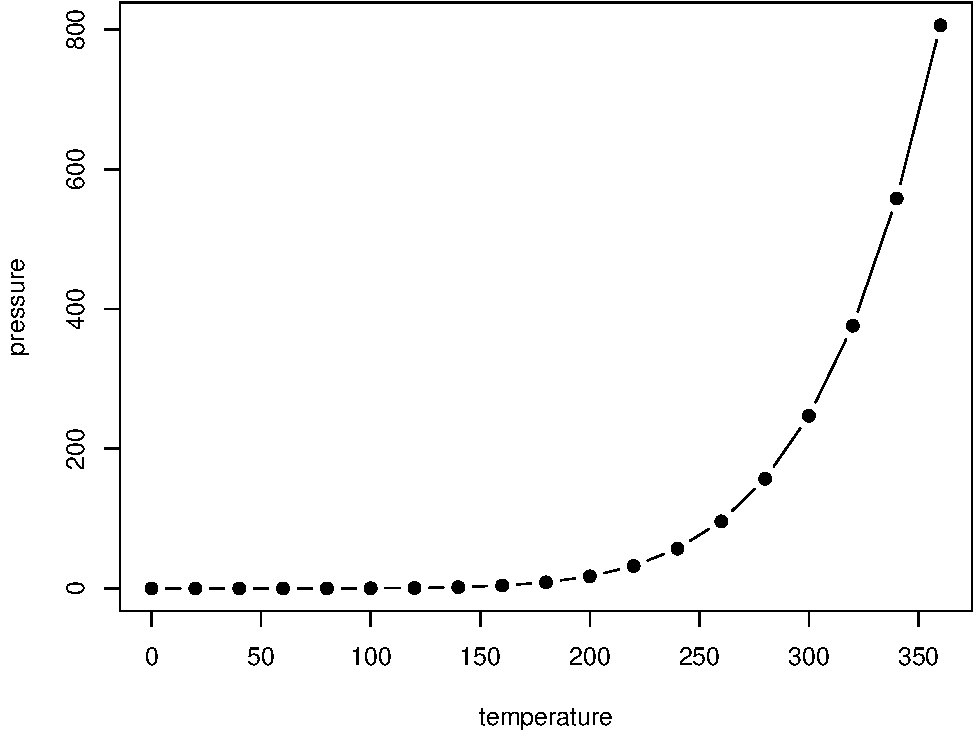
\includegraphics[width=0.8\linewidth]{AdvECTS_files/figure-latex/nice-fig-1} 

}

\caption{Here is a nice figure!}\label{fig:nice-fig}
\end{figure}

Reference a figure by its code chunk label with the \texttt{fig:} prefix, e.g., see Figure \ref{fig:nice-fig}. Similarly, you can reference tables generated from \texttt{knitr::kable()}, e.g., see Table \ref{tab:nice-tab}.

\begin{Shaded}
\begin{Highlighting}[]
\NormalTok{knitr}\SpecialCharTok{::}\FunctionTok{kable}\NormalTok{(}
  \FunctionTok{head}\NormalTok{(iris, }\DecValTok{20}\NormalTok{), }\AttributeTok{caption =} \StringTok{\textquotesingle{}Here is a nice table!\textquotesingle{}}\NormalTok{,}
  \AttributeTok{booktabs =} \ConstantTok{TRUE}
\NormalTok{)}
\end{Highlighting}
\end{Shaded}

\begin{table}

\caption{\label{tab:nice-tab}Here is a nice table!}
\centering
\begin{tabular}[t]{rrrrl}
\toprule
Sepal.Length & Sepal.Width & Petal.Length & Petal.Width & Species\\
\midrule
5.1 & 3.5 & 1.4 & 0.2 & setosa\\
4.9 & 3.0 & 1.4 & 0.2 & setosa\\
4.7 & 3.2 & 1.3 & 0.2 & setosa\\
4.6 & 3.1 & 1.5 & 0.2 & setosa\\
5.0 & 3.6 & 1.4 & 0.2 & setosa\\
\addlinespace
5.4 & 3.9 & 1.7 & 0.4 & setosa\\
4.6 & 3.4 & 1.4 & 0.3 & setosa\\
5.0 & 3.4 & 1.5 & 0.2 & setosa\\
4.4 & 2.9 & 1.4 & 0.2 & setosa\\
4.9 & 3.1 & 1.5 & 0.1 & setosa\\
\addlinespace
5.4 & 3.7 & 1.5 & 0.2 & setosa\\
4.8 & 3.4 & 1.6 & 0.2 & setosa\\
4.8 & 3.0 & 1.4 & 0.1 & setosa\\
4.3 & 3.0 & 1.1 & 0.1 & setosa\\
5.8 & 4.0 & 1.2 & 0.2 & setosa\\
\addlinespace
5.7 & 4.4 & 1.5 & 0.4 & setosa\\
5.4 & 3.9 & 1.3 & 0.4 & setosa\\
5.1 & 3.5 & 1.4 & 0.3 & setosa\\
5.7 & 3.8 & 1.7 & 0.3 & setosa\\
5.1 & 3.8 & 1.5 & 0.3 & setosa\\
\bottomrule
\end{tabular}
\end{table}

You can write citations, too. For example, we are using the \textbf{bookdown} package \citep{R-bookdown} in this sample book, which was built on top of R Markdown and \textbf{knitr} \citep{xie2015}.

Below is an example borrowed from \href{https://www.kellogg.northwestern.edu/faculty/petersen/htm/papers/se/test_data.htm}{Petersen}.

\begin{Shaded}
\begin{Highlighting}[]
\FunctionTok{library}\NormalTok{(sandwich)}
\DocumentationTok{\#\# Petersen\textquotesingle{}s data}
\FunctionTok{data}\NormalTok{(}\StringTok{"PetersenCL"}\NormalTok{, }\AttributeTok{package =} \StringTok{"sandwich"}\NormalTok{)}
\NormalTok{m }\OtherTok{\textless{}{-}} \FunctionTok{lm}\NormalTok{(y }\SpecialCharTok{\textasciitilde{}}\NormalTok{ x, }\AttributeTok{data =}\NormalTok{ PetersenCL)}

\DocumentationTok{\#\# clustered covariances}
\DocumentationTok{\#\# one{-}way}
\FunctionTok{vcovCL}\NormalTok{(m, }\AttributeTok{cluster =} \SpecialCharTok{\textasciitilde{}}\NormalTok{ firm)}
\end{Highlighting}
\end{Shaded}

\begin{verbatim}
##               (Intercept)             x
## (Intercept)  4.490702e-03 -6.473517e-05
## x           -6.473517e-05  2.559927e-03
\end{verbatim}

\begin{Shaded}
\begin{Highlighting}[]
\FunctionTok{vcovCL}\NormalTok{(m, }\AttributeTok{cluster =}\NormalTok{ PetersenCL}\SpecialCharTok{$}\NormalTok{firm) }\DocumentationTok{\#\# same}
\end{Highlighting}
\end{Shaded}

\begin{verbatim}
##               (Intercept)             x
## (Intercept)  4.490702e-03 -6.473517e-05
## x           -6.473517e-05  2.559927e-03
\end{verbatim}

\begin{Shaded}
\begin{Highlighting}[]
\DocumentationTok{\#\# one{-}way with HC2}
\FunctionTok{vcovCL}\NormalTok{(m, }\AttributeTok{cluster =} \SpecialCharTok{\textasciitilde{}}\NormalTok{ firm, }\AttributeTok{type =} \StringTok{"HC2"}\NormalTok{)}
\end{Highlighting}
\end{Shaded}

\begin{verbatim}
##               (Intercept)             x
## (Intercept)  4.494487e-03 -6.592912e-05
## x           -6.592912e-05  2.568236e-03
\end{verbatim}

\begin{Shaded}
\begin{Highlighting}[]
\DocumentationTok{\#\# two{-}way}
\FunctionTok{vcovCL}\NormalTok{(m, }\AttributeTok{cluster =} \SpecialCharTok{\textasciitilde{}}\NormalTok{ firm }\SpecialCharTok{+}\NormalTok{ year)}
\end{Highlighting}
\end{Shaded}

\begin{verbatim}
##               (Intercept)             x
## (Intercept)  4.233313e-03 -2.845344e-05
## x           -2.845344e-05  2.868462e-03
\end{verbatim}

\begin{Shaded}
\begin{Highlighting}[]
\FunctionTok{vcovCL}\NormalTok{(m, }\AttributeTok{cluster =}\NormalTok{ PetersenCL[, }\FunctionTok{c}\NormalTok{(}\StringTok{"firm"}\NormalTok{, }\StringTok{"year"}\NormalTok{)]) }\DocumentationTok{\#\# same}
\end{Highlighting}
\end{Shaded}

\begin{verbatim}
##               (Intercept)             x
## (Intercept)  4.233313e-03 -2.845344e-05
## x           -2.845344e-05  2.868462e-03
\end{verbatim}

XXXX

Sargan-Hansen () test. \citet{Sargan_1958} and \citet{Hansen_1982}

Durbin-Wu-Hausman test: \citet{Durbin_1954} / \citet{Wu_1973} / \citet{Hausman_1978}

\href{https://www.hds.utc.fr/~tdenoeux/dokuwiki/_media/en/kleibzeil_-_aer.pdf}{Use R!} is an excellent tutorial.
(notably for \texttt{plm} and the Arellano-Bond example, 140 UK firms)

Program evaluation (very good survey): \citet{Abadie_Cattaneo_2018}
Mostly harmless: \citet{angrist_mostly_2008}

Diff-in-Diff: \href{https://towardsdatascience.com/analyze-causal-effect-using-diff-in-diff-model-85e07b17e7b7}{Card and Krueger (1994)}

Diff-in-Diff:
\citet{Meyer_Viscusi_Durbin_1995}
with data in the \texttt{wooldridge} package. See \href{https://evalf20.classes.andrewheiss.com/example/diff-in-diff/}{this page}

\hypertarget{vector-auto-regressive-var-models}{%
\chapter{Vector Auto-Regressive (VAR) models}\label{vector-auto-regressive-var-models}}

\citet{Kilian_1998} See \href{https://rdrr.io/cran/VAR.etp/man/VAR.Boot.html}{this page}

Sign restrictions: \href{https://github.com/chrstdanne/VARsignR}{package}, \citet{Danne_2015}.

\citet{vars}

\citet{Stargazer}

\begin{Shaded}
\begin{Highlighting}[]
\FunctionTok{library}\NormalTok{(VAR.etp)}
\FunctionTok{library}\NormalTok{(vars) }\CommentTok{\#standard VAR models}
\FunctionTok{data}\NormalTok{(dat) }\CommentTok{\# part of VAR.etp package}
\NormalTok{a }\OtherTok{\textless{}{-}} \FunctionTok{VAR.Boot}\NormalTok{(dat,}\AttributeTok{p=}\DecValTok{2}\NormalTok{,}\AttributeTok{nb=}\DecValTok{200}\NormalTok{,}\AttributeTok{type=}\StringTok{"const"}\NormalTok{)}
\NormalTok{b }\OtherTok{\textless{}{-}} \FunctionTok{VAR}\NormalTok{(dat,}\AttributeTok{p=}\DecValTok{2}\NormalTok{)}
\FunctionTok{rbind}\NormalTok{(a}\SpecialCharTok{$}\NormalTok{coef[}\DecValTok{1}\NormalTok{,],(a}\SpecialCharTok{$}\NormalTok{coef}\SpecialCharTok{+}\NormalTok{a}\SpecialCharTok{$}\NormalTok{Bias)[}\DecValTok{1}\NormalTok{,],b}\SpecialCharTok{$}\NormalTok{varresult}\SpecialCharTok{$}\NormalTok{inv}\SpecialCharTok{$}\NormalTok{coefficients)}
\end{Highlighting}
\end{Shaded}

\begin{verbatim}
##         inv(-1)   inc(-1)  con(-1)    inv(-2)   inc(-2)   con(-2)       const
## [1,] -0.3177971 0.1318571 1.016190 -0.1310161 0.1495442 0.9587964 -0.01935124
## [2,] -0.3196310 0.1459888 0.961219 -0.1605511 0.1146050 0.9343938 -0.01672199
## [3,] -0.3196310 0.1459888 0.961219 -0.1605511 0.1146050 0.9343938 -0.01672199
\end{verbatim}

VARs are widely used in macroeconomic analysis. While simple and easy to estimate, they make it possible to conveniently capture the dynamics of complex multivariate systems. VAR popularity is notably due to \citet{Sims_1980}'s influential work. In economics, VAR models are often employed in order to identify \emph{structural} shocks. First, we will present VAR models. Second, we will study its \emph{structural} extension (SVAR models).

\begin{definition}[(S)VAR model]
\protect\hypertarget{def:SVAR}{}\label{def:SVAR}Let \(y_{t}\) denote a \(n \times1\) vector of random variables. Process \(y_{t}\) follows a \(p^{th}\)-order VAR if, for all \(t\), we have
\begin{eqnarray}
\begin{array}{rllll}
VAR:& y_t &=& c + \Phi_1 y_{t-1} + \dots + \Phi_p y_{t-p} + \varepsilon_t,& \varepsilon_t:\mbox{ (correlated) innovation}\\
SVAR:& y_t &=& c + \Phi_1 y_{t-1} + \dots + \Phi_p y_{t-p} + B \eta_t,& \eta_t:\mbox{ ($\bot$) structural shock},
\end{array}\label{eq:yVAR}
\end{eqnarray}
with \(\varepsilon_t = B\eta_t\). We assume that \(\{\eta_{t}\}\) is a white noise sequence whose components are are mutually and serially independent.
\end{definition}

The first line of Eq. \eqref{eq:yVAR} corresponds to the \textbf{reduced-form} of the VAR model (\textbf{structural form} for the second line).

Eq. \eqref{eq:yVAR} can also be written:
\[
y_{t}=c+\Phi(L)y_{t-1}+\varepsilon_{t},
\]
with \(\Phi(L) = \Phi_1 + \Phi_2 L + \dots + \Phi_p L^{p-1}\).

Consequently:
\[
y_{t}\mid y_{t-1},y_{t-2},\ldots,y_{-p+1}\sim \mathcal{N}(c+\Phi_{1}y_{t-1}+\ldots\Phi_{p}y_{t-p},\Omega).
\]

Using \citet{Hamilton_1994}'s notations, denote with \(\Pi\) the matrix \(\left[\begin{array}{ccccc} c & \Phi_{1} & \Phi_{2} & \ldots & \Phi_{p}\end{array}\right]'\) and with \(x_{t}\) the vector \(\left[\begin{array}{ccccc} 1 & y'_{t-1} & y'_{t-2} & \ldots & y'_{t-p}\end{array}\right]'\), we have:
\begin{equation}
y_{t}= \Pi'x_{t} + \varepsilon_{t}. \label{eq:PIVAR}
\end{equation}
The previous representation is convenient to discuss the estimation of the VAR model, as parameters are gathered in two matrices only: \(\Pi\) and \(\Omega\).

\hypertarget{var-estimation}{%
\subsection{VAR estimation}\label{var-estimation}}

Let us start with the case where the shocks are Gaussian.

\begin{proposition}[MLE of a Gaussian VAR]
\protect\hypertarget{prp:estimVARGaussian}{}\label{prp:estimVARGaussian}If \(y_t\) follows a VAR(p) (see Definition \ref{def:SVAR}), and if \(\varepsilon_t \sim \,i.i.d.\,\mathcal{N}(0,\Omega)\), then the ML estimate of \(\Pi\), denoted by \(\hat{\Pi}\) (see Eq. \eqref{eq:PIVAR}), is given by
\begin{equation}
\hat{\Pi}=\left[\sum_{t=1}^{T}x_{t}x'_{t}\right]^{-1}\left[\sum_{t=1}^{T}y_{t}'x_{t}\right]= (\mathbf{X}'\mathbf{X})^{-1}\mathbf{X}'\mathbf{y},\label{eq:Pi}
\end{equation}
where \(\mathbf{X}\) is the \(T \times (np)\) matrix whose \(t^{th}\) row is \(x_t\) and where \(\mathbf{y}\) is the \(T \times n\) matrix whose \(t^{th}\) row is \(y_{t}'\).

That is, the \(i^{th}\) column of \(\hat{\Pi}\) (\(b_i\), say) is the OLS estimate of \(\beta_i\), where:
\begin{equation}
y_{i,t} = \beta_i'x_t + \varepsilon_{i,t},\label{eq:betayx}
\end{equation}
(i.e., \(\beta_i' = [c_i,\phi_{i,1}',\dots,\phi_{i,p}']'\)).

The ML estimate of \(\Omega\), denoted by \(\hat{\Omega}\), coincides with the sample covariance matrix of the \(n\) series of the OLS residuals in Eq. \eqref{eq:betayx}, i.e.:
\begin{equation}
\hat{\Omega} = \frac{1}{T} \sum_{i=1}^T \hat{\varepsilon}_t\hat{\varepsilon}_t',\quad\mbox{with } \hat{\varepsilon}_t= y_t - \hat{\Pi}'x_t.
\end{equation}

The asymptotic distributions of these estimators are the ones resulting from standard OLS formula.
\end{proposition}

\begin{proof}
See Appendix \ref{estimVARGaussian}.
\end{proof}

As stated by Proposition \ref{OLSVAR}, when the shocks are not Gaussian, then the OLS regressions still provide consistent estimates of the model parameters. However, since \(x_t\) correlates to \(\varepsilon_s\) for \(s<t\), the OLS estimator \(\mathbf{b}_i\) of \(\boldsymbol\beta_i\) is biased in small sample. (That is also the case for the ML estimator.)

Indeed, denoting by \(\boldsymbol\varepsilon_i\) the \(T \times 1\) vector of \(\varepsilon_{i,t}\)'s, and using the notations of \(b_i\) and \(\beta_i\) introduced in Proposition \ref{prp:estimVARGaussian}, we have:
\begin{equation}
\mathbf{b}_i = \beta_i + (\mathbf{X}'\mathbf{X})^{-1}\mathbf{X}'\boldsymbol\varepsilon_i.\label{eq:olsar1}
\end{equation}
We have non-zero correlation between \(x_t\) and \(\varepsilon_{i,s}\) for \(s<t\) and, therefore, \(\mathbb{E}[(\mathbf{X}'\mathbf{X})^{-1}\mathbf{X}'\boldsymbol\varepsilon_i] \ne 0\).

However, when \(y_t\) is covariance stationary, then \(\frac{1}{n}\mathbf{X}'\mathbf{X}\) converges to a positive definite matrix \(\mathbf{Q}\), and \(\frac{1}{n}X'\boldsymbol\varepsilon_i\) converges to 0. Hence \(\mathbf{b}_i \overset{p}{\rightarrow} \beta_i\). More precisely:

\begin{proposition}[Asymptotic distribution of the OLS estimate of $\beta_i$]
\protect\hypertarget{prp:OLSVAR}{}\label{prp:OLSVAR}If \(y_t\) follows a VAR model, as defined in Definition \ref{def:SVAR}, we have:
\[
\sqrt{T}(\mathbf{b}_i-\beta_i) =  \underbrace{\left[\frac{1}{T}\sum_{t=p}^T x_t x_t' \right]^{-1}}_{\overset{p}{\rightarrow} \mathbf{Q}^{-1}}
\underbrace{\sqrt{T} \left[\frac{1}{T}\sum_{t=1}^T x_t\varepsilon_{i,t} \right]}_{\overset{d}{\rightarrow} \mathcal{N}(0,\sigma_i^2\mathbf{Q})},
\]
where \(\sigma_i = \mathbb{V}ar(\varepsilon_{i,t})\) and where \(\mathbf{Q} = \mbox{plim }\frac{1}{T}\sum_{t=p}^T x_t x_t'\) is given by:
\begin{equation}
\mathbf{Q} = \left[
\begin{array}{ccccc}
1 & \mu' &\mu' & \dots & \mu' \\
\mu & \gamma_0 + \mu\mu' & \gamma_1 + \mu\mu' & \dots & \gamma_{p-1} + \mu\mu'\\
\mu & \gamma_1 + \mu\mu' & \gamma_0 + \mu\mu' & \dots & \gamma_{p-2} + \mu\mu'\\
\vdots &\vdots &\vdots &\dots &\vdots \\
\mu & \gamma_{p-1} + \mu\mu' & \gamma_{p-2} + \mu\mu' & \dots & \gamma_{0} + \mu\mu'
\end{array}
\right].\label{eq:Qols}
\end{equation}
\end{proposition}

\begin{proof}
See Appendix \ref{OLSVAR}.
\end{proof}

The following proposition extends the previous proposition and includes covariances between different \(\beta_i\)'s as well as the asymptotic distribution of the ML estimates of \(\Omega\).

\begin{proposition}[Asymptotic distribution of the OLS estimates]
\protect\hypertarget{prp:OLSVAR2}{}\label{prp:OLSVAR2}If \(y_t\) follows a VAR model, as defined in Definition \ref{def:SVAR}, we have:
\begin{equation}
\sqrt{T}\left[
\begin{array}{c}
vec(\hat\Pi - \Pi)\\
vec(\hat\Omega - \Omega)
\end{array}
\right]
\sim \mathcal{N}\left(0,
\left[
\begin{array}{cc}
\Omega \otimes \mathbf{Q}^{-1} & 0\\
0 & \Sigma_{22}
\end{array}
\right]\right),\label{eq:asymptPi}
\end{equation}
where the component of \(\Sigma_{22}\) corresponding to the covariance between \(\hat\sigma_{i,j}\) and \(\hat\sigma_{k,l}\) (for \(i,j,l,m \in \{1,\dots,n\}^4\)) is equal to \(\sigma_{i,l}\sigma_{j,m}+\sigma_{i,m}\sigma_{j,l}\).
\end{proposition}

\begin{proof}
See \citet{Hamilton_1994}, Appendix of Chapter 11.
\end{proof}

Naturally, in practice, \(\Omega\) is replaced by \(\hat{\Omega}\), \(Q\) is replaced with \(\hat{\mathbf{Q}} = \frac{1}{T}\sum_{t=p}^T x_t x_t'\) and \(\Sigma\) with the matrix whose components are of the form \(\hat\sigma_{i,l}\hat\sigma_{j,m}+\hat\sigma_{i,m}\hat\sigma_{j,l}\), where the \(\hat\sigma_{i,l}\)'s are the components of \(\hat\Omega\).

The simplicity of the VAR framework and the tractability of its MLE open the way to convenient econometric testing. Let's illustrate this with the likelihood ratio test. The maximum value achieved by the MLE is
\[
\log\mathcal{L}(Y_{T};\hat{\Pi},\hat{\Omega}) = -\frac{Tn}{2}\log(2\pi)+\frac{T}{2}\log\left|\hat{\Omega}^{-1}\right| -\frac{1}{2}\sum_{t=1}^{T}\left[\hat{\varepsilon}_{t}'\hat{\Omega}^{-1}\hat{\varepsilon}_{t}\right].
\]
The last term is:
\begin{eqnarray*}
\sum_{t=1}^{T}\hat{\varepsilon}_{t}'\hat{\Omega}^{-1}\hat{\varepsilon}_{t} &=& \mbox{Tr}\left[\sum_{t=1}^{T}\hat{\varepsilon}_{t}'\hat{\Omega}^{-1}\hat{\varepsilon}_{t}\right] = \mbox{Tr}\left[\sum_{t=1}^{T}\hat{\Omega}^{-1}\hat{\varepsilon}_{t}\hat{\varepsilon}_{t}'\right]\\
&=&\mbox{Tr}\left[\hat{\Omega}^{-1}\sum_{t=1}^{T}\hat{\varepsilon}_{t}\hat{\varepsilon}_{t}'\right] = \mbox{Tr}\left[\hat{\Omega}^{-1}\left(T\hat{\Omega}\right)\right]=Tn.
\end{eqnarray*}
Therefore, the optimized log-likelihood is simply obtained by:
\begin{equation}
\log\mathcal{L}(Y_{T};\hat{\Pi},\hat{\Omega})=-(Tn/2)\log(2\pi)+(T/2)\log\left|\hat{\Omega}^{-1}\right|-Tn/2.\label{eq:optimzedLogL}
\end{equation}

Assume that we want to test the null hypothesis that a set of variables follows a VAR(\(p_{0}\)) against the alternative
specification of \(p_{1}\) (\(>p_{0}\)).

Let us denote by \(\hat{L}_{0}\) and \(\hat{L}_{1}\) the maximum log-likelihoods obtained with \(p_{0}\) and \(p_{1}\) lags, respectively.

Under the null hypothesis (\(H_0\): \(p=p_0\)), we have:
\begin{eqnarray*}
2\left(\hat{L}_{1}-\hat{L}_{0}\right)&=&T\left(\log\left|\hat{\Omega}_{1}^{-1}\right|-\log\left|\hat{\Omega}_{0}^{-1}\right|\right)  \sim \chi^2(n^{2}(p_{1}-p_{0})).
\end{eqnarray*}

\textbf{Block exogeneity}

Let's decompose \(y_t\) into two subvectors \(y^{(1)}_{t}\) (\(n_1 \times 1\)) and \(y^{(2)}_{t}\) (\(n_2 \times 1\)), with \(y_t' = [{y^{(1)}_{t}}',{y^{(2)}_{t}}']\) (and therefore \(n=n_1 +n_2\)), such that:
\[
\left[
\begin{array}{c}
y^{(1)}_{t}\\
y^{(2)}_{t}
\end{array}
\right] = \left[
\begin{array}{cc}
\Phi^{(1,1)} & \Phi^{(1,2)}\\
\Phi^{(2,1)} & \Phi^{(2,2)}
\end{array}
\right]
\left[
\begin{array}{c}
y^{(1)}_{t-1}\\
y^{(2)}_{t-1}
\end{array}
\right] + \varepsilon_t.
\]
One can easily test for block exogeneity of \(y_t^{(2)}\) (say). The null assumption ca n be expressed as \(\Phi^{(2,1)}=0\) and \(\Sigma^{(2,1)}=0\).

\textbf{Lag selection}

In a VAR, adding lags consumes numerous degrees of freedom: with \(p\) lags, each of the \(n\) equations in the VAR contains \(n\times p\) coefficients plus the intercept term.

Adding lags improve in-sample fit, but is likely to result in over-parameterization and affect the \{\color{blue}out-of-sample\} prediction performance.

To select appropriate lag length, so-called \textbf{selection criteria} can be used (see Definition \ref{def:infocriteria}). These criteria have to be minimized. That is, the best specification is the one giving the lowest criteria.

In the context of VAR models, using Eq. \eqref{eq:optimzedLogL}, we have:
\begin{eqnarray*}
AIC & = & cst + \log\left|\hat{\Omega}\right|+\frac{2}{T}N\\
BIC & = & cst + \log\left|\hat{\Omega}\right|+\frac{\log T}{T}N,
\end{eqnarray*}
where \(N=p \times n^{2}\).

\textbf{Companion Form and Stability of a VAR process}

Let us introduce vector \(y_{t}^{*}\), whihc stacks the last \(p\) values of \(y_t\):
\[
y_{t}^{*}=\left[\begin{array}{cccc}
y'_{t} & y'_{t-1} & \ldots & y'_{t-p+1}\end{array}\right]^{'},
\]
Eq. \eqref{eq:yVAR} can then be rewritten in its companion form:
\begin{equation}
y_{t}^{*} =
\underbrace{\left[\begin{array}{c}
c\\
0\\
\vdots\\
0\end{array}\right]}_{=c^*}+
\underbrace{\left[\begin{array}{cccc}
\Phi_{1} & \Phi_{2} & \cdots & \Phi_{p}\\
I & 0 & \cdots & 0\\
0 & \ddots & 0 & 0\\
0 & 0 & I & 0\end{array}\right]}_{=\Phi}
y_{t-1}^{*}+
\underbrace{\left[\begin{array}{c}
\varepsilon_{t}\\
0\\
\vdots\\
0\end{array}\right]}_{\varepsilon_t^*}\label{eq:ystarVAR}
\end{equation}

Matrices \(\Phi\) and \(\Sigma^* = \mathbb{V}ar(\varepsilon_t^*)\) are of dimension \(np \times np\). \(\Sigma^*\) is filled with zeros, except the \(n\times n\) upper-left block that is equal to \(\Sigma = \mathbb{V}ar(\varepsilon_t)\).

We then have:
\begin{eqnarray*}
y_{t}^{*} & = & c^{*}+\Phi\left(c^{*}+\Phi y_{t-2}^{*}+\varepsilon_{t-1}^{*}\right)+\varepsilon_{t}^{*} \nonumber \\
& = & c^{*}+\varepsilon_{t}^{*}+\Phi(c^{*}+\varepsilon_{t-1}^{*})+\ldots+\Phi^{k}(c^{*}+\varepsilon_{t-k}^{*})+\Phi^k y_{t-k}^{*}.
\end{eqnarray*}

If the eigenvalues of \(\Phi\) are strictly within the unit circle, then \(\Phi^k\) geometrically decays to the zero matrix and we get the following Wold decomposition for \(y_t\):
\begin{eqnarray}
y_{t}^{*}  & = & c^{*}+\varepsilon_{t}^{*}+\Phi(c^{*}+\varepsilon_{t-1}^{*})+\ldots+\Phi^{k}(c^{*}+\varepsilon_{t-k}^{*})+\ldots \nonumber \\
& = & \mu^{*} +\varepsilon_{t}^{*}+\Phi\varepsilon_{t-1}^{*}+\ldots+\Phi^{k}\varepsilon_{t-k}^{*}+\ldots,\label{eq:VARstar}
\end{eqnarray}
where \(\mu^* = (I - \Phi)^{-1} c^*\).

(It can also be seen that \(\mu^{*} = [\mu',\dots,\mu']'\), where \(\mu = (I - \Phi_1 - \dots - \Phi_p)^{-1}c\)).

The unconditional variance of \(y_t\) can be derived from Eq. \eqref{eq:VARstar}, exploiting the fact that the \(\varepsilon_{t}^{*}\) are serially uncorrelated:
\[
\mathbb{V}ar(y_t^*)=\Omega^*+\Phi\Omega^*\Phi'+\ldots+\Phi^{k}\Omega^*\Phi'^{k}+\ldots,
\]
with \(\mathbb{V}ar(\varepsilon_t^*)=\Omega^*\).

The unconditional variance of \(y_t\) is the upper-left \(n\times n\) block of matrix \(\mathbb{V}ar(y_t^*)\).

Eq. \eqref{eq:VARstar} also implies that the \(\Psi_k\) matrices defining the IRFs (see Eq. \eqref{eq:InfMA}) are given by: \(\Psi_k = \widetilde{\Phi^k}B\), where \(\widetilde{\Phi^k}\) is the upper-left matrix block of \(\Phi^k\).

\textbf{Granger Causality}

\citet{Granger_1969} developed a method to explore \textbf{causal relationships} among variables. The approach consists in determining whether the past values of \(y_{1,t}\) can help explain the current \(y_{2,t}\) (beyond the information already included in the past values of \(y_{2,t}\)).

Formally, let us denote three information sets:
\begin{eqnarray*}
\mathcal{I}_{1,t} & = & \left\{ y_{1,t},y_{1,t-1},\ldots\right\} \\
\mathcal{I}_{2,t} & = & \left\{ y_{2,t},y_{2,t-1},\ldots\right\} \\
\mathcal{I}_{t} & = & \left\{ y_{1,t},y_{1,t-1},\ldots y_{2,t},y_{2,t-1},\ldots\right\}.
\end{eqnarray*}
We say that \(y_{1,t}\) Granger-causes \(y_{2,t}\) if
\[
\mathbb{E}\left[y_{2,t}\mid \mathcal{I}_{2,t-1}\right]\neq \mathbb{E}\left[y_{2,t}\mid \mathcal{I}_{t-1}\right].
\]

To get the intuition behind the testing procedure, consider the following
bivariate VAR(\(p\)) process:
\begin{eqnarray*}
y_{1,t} & = & c_1+\Sigma_{i=1}^{p}\Phi_i^{(11)}y_{1,t-i}+\Sigma_{i=1}^{p}\Phi_i^{(12)}y_{2,t-i}+\varepsilon_{1,t}\\
y_{2,t} & = & c_2+\Sigma_{i=1}^{p}\Phi_i^{(21)}y_{1,t-i}+\Sigma_{i=1}^{p}\Phi_i^{(22)}y_{2,t-i}+\varepsilon_{2,t},
\end{eqnarray*}
where \(\Phi_k^{(ij)}\) denotes the element \((i,j)\) of \(\Phi_k\).

Then, \(y_{1,t}\) is said not to Granger-cause \(y_{2,t}\) if
\[
\Phi_1^{(21)}=\Phi_2^{(21)}=\ldots=\Phi_p^{(21)}=0.
\]
Therefore the hypothesis testing is
\[
\begin{cases}
H_{0}: & \Phi_1^{(21)}=\Phi_2^{(21)}=\ldots=\Phi_p^{(21)}=0\\
H_{1}: & \Phi_1^{(21)}\neq0\mbox{ or }\Phi_2^{(21)}\neq0\mbox{ or}\ldots\Phi_p^{(21)}\neq0.\end{cases}
\]
Loosely speaking, we reject \(H_{0}\) if some of the coefficients on the lagged \(y_{1,t}\)'s are statistically significant. Formally, this can be tested using the \(F\)-test or asymptotic chi-square test. The \(F\)-statistic is
\[
F=\frac{(RSS-USS)/p}{USS/(T-2p-1)},
\]
where RSS is the Restricted sum of squared residuals and USS is the Unrestricted sum of squared residuals. Under \(H_{0}\), the \(F\)-statistic is distributed as \(\mathcal{F}(p,T-2p-1)\).

Note that \(pF\underset{T \rightarrow \infty}{\rightarrow}\chi^{2}(p)\). Therefore, for large samples and under \(H_0\):
\[
F \sim \chi^{2}(p)/p.
\]

\textbf{Factor-Augmented VAR (FAVAR)}

VAR models are subject to the curse of dimensionality: If \(n\), is large, then the number of parameters (in \(n^2\)) explodes.

In the case where one suspects that the \(y_{i,t}\)'s are mainly driven by a small number of random sources, a \textbf{factor structure} may be imposed (\citet{Bernanke_Boivin_Eliasz_2005}).

Let us denote by \(f_t\) a \(k\)-dimensional vector of latent factors accounting for important shares of the variances of the \(y_{i,t}\)'s (with \(k \ll n\)) and by \(x_t\) is a small \(q\)-dimensional subset of \(y_t\) (with \(q \ll n\)). The following factor structure is posited:
\[
y_t = \Lambda^f f_t + \Lambda^x x_t + e_t,
\]
where the \(e_t\) are ``small'\,' serially and mutually i.i.d. error terms.

The model is complemented by positing a VAR dynamics for \([f_t',x_t']'\):
\begin{equation}
\left[\begin{array}{c}f_t\\x_t\end{array}\right] = \Phi(L)\left[\begin{array}{c}f_{t-1}\\x_{t-1}\end{array}\right] + v_t.\label{eq:FAVAR}
\end{equation}

\(f_t\) e.g.~\(\equiv\) the first \(k\) principal components of \(y_t\).

Standard identification techniques of structural shocks can be employed in Eq. \eqref{eq:FAVAR}: Cholesky approach can be used for instance if the last component of \(x_t\) is the short-term interest rate and if it is assumed that a MP shock has no contemporaneous impact on other macro-variables (in \(y_t\)).

\hypertarget{identification-problem-and-standard-identification-techniques}{%
\section{Identification Problem and Standard Identification Techniques}\label{identification-problem-and-standard-identification-techniques}}

\textbf{The Identification Issue}*

In the previous section, we have seen how to estimate \(\Omega\) and the \(\Phi_k\) matrices in the context of a VAR model. But the IRFs are functions of \(B\) and the \(\Phi_k\)'s, not of \(\Omega\) the \(\Phi_k\)'s. We have \(\Omega = BB'\), but this is not sufficient to recover \(B\).

Indeed, seen a system of equations whose unknowns are the \(b_{i,j}\)'s (components of \(B\)), the system \(\Omega = BB'\) contains only \(n(n+1)/2\) linearly independent equations. Example for \(n=2\):
\begin{eqnarray*}
&&\left[
\begin{array}{cc}
\omega_{11} & \omega_{12} \\
\omega_{12} & \omega_{22}
\end{array}
\right] = \left[
\begin{array}{cc}
b_{11} & b_{12} \\
b_{21} & b_{22}
\end{array}
\right]\left[
\begin{array}{cc}
b_{11} & b_{21} \\
b_{12} & b_{22}
\end{array}
\right]\\
&\Leftrightarrow&\left[
\begin{array}{cc}
\omega_{11} & \omega_{12} \\
\omega_{12} & \omega_{22}
\end{array}
\right] = \left[
\begin{array}{cc}
b_{11}^2+b_{12}^2 & {\color{red}b_{11}b_{21}+b_{12}b_{22}} \\
{\color{red}b_{11}b_{21}+b_{12}b_{22}} & b_{22}^2 + b_{21}^2
\end{array}
\right].
\end{eqnarray*}

We have 3 linearly independent equations but 4 unknowns. Therefore, \(B\) is not identified based on second-order moments. Additional restrictions are required to identify \(B\).

This section covers two standard identification schemes: \textbf{short-run} and \textbf{long-run} restrictions:

\begin{enumerate}
\def\labelenumi{\arabic{enumi}.}
\tightlist
\item
  a \textbf{short-run restriction (SRR)} prevents a structural shock from affecting an endogenous variable contemporaneously.
\end{enumerate}

\begin{itemize}
\tightlist
\item
  Easy to implement: the appropriate entries of \(B\) are set to 0.
\item
  Particular case: \textbf{Cholesky, or recursive approach}.
\item
  Examples: \citet{BERNANKE198649}, \citet{Sims_1986}, \citet{Gali_1992}, \citet{RubioRamirez_et_al_2010}.
\end{itemize}

\begin{enumerate}
\def\labelenumi{\arabic{enumi}.}
\setcounter{enumi}{1}
\tightlist
\item
  a \textbf{long-run restriction (LRR)} prevents a structural shock from having a cumulative impact on one of the endogenous variables.
\end{enumerate}

\begin{itemize}
\tightlist
\item
  Additional computations are required to implement this. One needs to compute the cumulative effect of one of the structural shocks \(u_{t}\) on one of the endogenous variable.
\item
  Examples: \citet{Blanchard_Quah_1989}, \citet{Faust_Leeper_1997}, \citet{Gali_1999}, \citet{Erceg_et_al_2005}, \citet{NBERc11177}.
\end{itemize}

The two approaches can be combined (see, e.g., \citet{Gerlach_Smets_1995}).

\textbf{A Simple Example}

Consider the following stylized economic dynamics:
\begin{equation}
\begin{array}{clll}
g_{t}&=& \bar{g}-\lambda(i_{t-1}-\mathbb{E}_{t-1}\pi_{t})+ \underbrace{{\color{blue}\sigma_d \eta_{d,t}}}_{\mbox{demand shock}}& (\mbox{IS curve})\\
\Delta \pi_{t} & = & \beta (g_{t} - \bar{g})+ \underbrace{{\color{blue}\sigma_{\pi} \eta_{\pi,t}}}_{\mbox{cost push shock}} & (\mbox{Phillips curve})\\
i_{t} & = & \rho i_{t-1} + \left[ \gamma_\pi \mathbb{E}_{t}\pi_{t+1}  + \gamma_g (g_{t} - \bar{g}) \right]\\
&& \qquad \qquad+\underbrace{{\color{blue}\sigma_{mp} \eta_{mp,t}}}_{\mbox{Mon. Pol. shock}} & (\mbox{Taylor rule}),
\end{array}\label{eq:systemI}
\end{equation}
where:
\begin{equation}
\eta_t = 
\left[
\begin{array}{c}
\eta_{\pi,t}\\
\eta_{d,t}\\
\eta_{mp,t}
\end{array}
\right]
\sim i.i.d.\,\mathcal{N}(0,I).\label{eq:covU}
\end{equation}

Vector \(\eta_t\) is a vector of Gaussian \{\color{blue}structural shocks\}, mutually and serially independent.

On date \(t\):

\begin{itemize}
\tightlist
\item
  \(g_t\) is contemporaneously affected by \(\eta_{d,t}\) only;
\item
  \(\pi_t\) is contemporaneously affected by \(\eta_{\pi,t}\) and \(\eta_{d,t}\);
\item
  \(i_t\) is contemporaneously affected by \(\eta_{mp,t}\), \(\eta_{\pi,t}\) and \(\eta_{d,t}\).
\end{itemize}

System \eqref{eq:systemI} could be rewritten in the form:
\begin{equation}
\left[\begin{array}{c}
d_t\\
\pi_t\\
i_t
\end{array}\right]
= \Phi(L)
\left[\begin{array}{c}
d_{t-1}\\
\pi_{t-1}\\
i_{t-1} +
\end{array}\right] +\underbrace{\underbrace{
\left[
\begin{array}{ccc}
0 & \bullet & 0 \\
\bullet & \bullet & 0 \\
\bullet & \bullet & \bullet
\end{array}
\right]}_{=B} \eta_t}_{=\varepsilon_t}\label{eq:BBBB}
\end{equation}

This is the \textbf{reduced-form} of the model. This representation suggests three additional restrictions on the entries of \(B\); the latter matrix is therefore identified (up to the signs of its columns) as soon as \(\Omega = BB'\) is known.

There are particular cases in which some well-known matrix decompositions of \(\mathbb{V}ar(\varepsilon_t)=\Omega_\varepsilon\) can be used to easily estimate some specific SVAR.

Consider the following context:

\begin{itemize}
\tightlist
\item
  A first shock (say, \(\eta_{n_1,t}\)) can affect instantaneously
  (i.e., on date \(t\)) only one of the endogenous variable (say, \(y_{n_1,t}\));
\item
  A second shock (say, \(\eta_{n_2,t}\)) can affect instantaneously
  (i.e., on date \(t\)) the first two endogenous variables (say, \(y_{n_1,t}\)
  and \(y_{n_2,t}\));
\item
  \ldots{}
\end{itemize}

This implies (1) that column \(n_1\) of \(B\) has only 1 non-zero entry (this is the \(n_1^{th}\) entry), (2) that column \(n_2\) of \(B\) has 2 non-zero entries (the \(n_1^{th}\) and the \(n_2^{th}\) ones), \ldots{}

Without loss of generality, we can set \(n_1=n\), \(n_2=n-1\), \ldots{} In this context, matrix \(B\) is lower triangular.

The Cholesky decomposition of \(\Omega_{\varepsilon}\) then provides an appropriate estimate of \(B\), that is a lower triangular matrix \(B\) that is such that:
\[
\Omega_\varepsilon = BB'.
\]

For instance, \citet{DEDOLA20051543} estimate 5 structural VAR models for the US, the UK, Germany, France and Italy to analyse the monetary-policy transmission mechanisms. They estimate SVAR(5) models over the period 1975-1997. The shock-identification scheme is based on Cholesky decompositions, the ordering of the endogenous variables being: the industrial production, the consumer price index, a commodity price index, the short-term rate, monetary aggregate and the effective exchange rate (except for the US). This ordering implies that monetary policy reacts to the shocks affecting
the first three variables but that the latter react to monetary policy shocks with a one-period lag.

Importantly, the Cholesky approach can be useful if you are essentially interested in one structural shock. This was the case, e.g., of \citet{Christiano_Eichenbaum_Evans_1996}. Their identification is based on the following relationship between \(\varepsilon_t\) and \(\eta_t\):
\[
\left[\begin{array}{c}
\boldsymbol\varepsilon_{S,t}\\
\varepsilon_{r,t}\\
\boldsymbol\varepsilon_{F,t}
\end{array}\right] =
\left[\begin{array}{ccc}
B_{SS} & 0 & 0 \\
B_{rS} & B_{rr} & 0 \\
B_{FS} & B_{Fr} & B_{FF}
\end{array}\right]
\left[\begin{array}{c}
\boldsymbol\eta_{S,t}\\
\eta_{r,t}\\
\boldsymbol\eta_{F,t}
\end{array}\right],
\]
where \(S\), \(r\) and \(F\) respectively correspond to \emph{slow-moving variables}, the policy variable (short-term rate) and \emph{fast-moving variables}. While \(\eta_{r,t}\) is scalar, \(\boldsymbol\eta_{S,t}\) and \(\boldsymbol\eta_{F,t}\) may be vectors. The space spanned by \(\boldsymbol\varepsilon_{S,t}\) is the same as that spanned by \(\boldsymbol\eta_{S,t}\). As a result, because \(\varepsilon_{r,t}\) is a linear combination of \(\eta_{r,t}\) and \(\boldsymbol\eta_{S,t}\) (which are \(\perp\)), it comes that the \(B_{rr}\eta_{r,t}\)'s are the (population) residuals in the regression of \(\varepsilon_{r,t}\) on \(\boldsymbol\varepsilon_{S,t}\). Because \(\mathbb{V}ar(\eta_{r,t})=1\), \(B_{rr}\) is given by the square root of the variance of \(B_{rr}\eta_{r,t}\). \(B_{F,r}\) is finally obtained by regressing the components of \(\boldsymbol\varepsilon_{F,t}\) on \(\eta_{r,t}\).

An equivalent approach consists in computing the Cholesky decomposition of \(BB'\) and keep only the column corresponding to the policy variable.

\textbf{Long-run restrictions}

A second type of restriction relates to the long-run influence of a shock on an endogenous variable. Let us consider for instance a structural shock that is assumed to have no ``long-run influence'' on GDP. How to express this? The long-run change in GDP can be expressed as \(GDP_{t+h} - GDP_t\), with \(h\) large. Note further that:
\[
GDP_{t+h} - GDP_t = \Delta GDP_{t+h} +\Delta GDP_{t+h-1} + \dots + \Delta GDP_{t+1}.
\]
Hence, the fact that a given structural shock (\(\eta_{i,t}\), say) has no long-run influence on GDP means that
\[
\lim_{h\rightarrow\infty}\frac{\partial GDP_{t+h}}{\partial \eta_{i,t}} = \lim_{h\rightarrow\infty} \frac{\partial}{\partial \eta_{i,t}}\left(\sum_{k=1}^h \Delta  GDP_{t+k}\right)= 0.
\]

This can be easily formulated as a function of \(B\) when \(y_t\) (including \(\Delta GDP_t\)) follows a VAR(MA) process.

As was shown previously (Eq. \eqref{eq:ystarVAR}), one can always write a VAR(\(p\)) as a VAR(1). Consequently, let us focus on the VAR(1) case:
\begin{eqnarray}
y_{t} &=& c+\Phi y_{t-1}+\varepsilon_{t}\\
& = & c+\varepsilon_{t}+\Phi(c+\varepsilon_{t-1})+\ldots+\Phi^{k}(c+\varepsilon_{t-k})+\ldots \nonumber \\
& = & \mu +\varepsilon_{t}+\Phi\varepsilon_{t-1}+\ldots+\Phi^{k}\varepsilon_{t-k}+\ldots \\
& = & \mu +B\eta_{t}+\Phi B\eta_{t-1}+\ldots+\Phi^{k}B\eta_{t-k}+\ldots,
\end{eqnarray}

The sequence of shocks \(\{\eta_t\}\) determines the sequence \(\{y_t\}\). What if \(\{\eta_t\}\) is replaced by \(\{\tilde{\eta}_t\}\), where \(\tilde{\eta}_t=\eta_t\) if \(t \ne s\) and \(\tilde{\eta}_s=\eta_s + \gamma\)?

Assume \(\{\tilde{y}_t\}\) is the associated ``perturbated'' sequence. We have \(\tilde{y}_t = y_t\) if \(t<s\). For \(t \ge s\), the Wold decomposition of \(\{\tilde{y}_t\}\) implies:
\[
\tilde{y}_t = y_t + \Phi^{t-s} B \gamma.
\]

Therefore, the cumulative impact of \(\gamma\) on \(\tilde{y}_t\) will be (for \(t \ge s\)):
\begin{eqnarray}
(\tilde{y}_t - y_t) +  (\tilde{y}_{t-1} - y_{t-1}) + \dots +  (\tilde{y}_s - y_s) &=& \nonumber \\
(Id + \Phi + \Phi^2 + \dots + \Phi^{t-s}) B \gamma.&& \label{eq:cumul}
\end{eqnarray}

Consider a shock on \(\eta_{1,t}\), with a magnitude of \(1\). This shock is \(\gamma = [1,0,\dots,0]'\). Given Eq. @ref\{eq:cumul), the long-run cumulative effect of this shock on the endogenous variables is given by:
\[
(Id+\Phi+\ldots+\Phi^{k}+\ldots)B\left[\begin{array}{c}
1\\
0\\
\vdots\\
0\end{array}\right],
\]
that is the first column of \(\Theta \equiv (I+\Phi+\ldots+\Phi^{k}+\ldots)B\).

In this context, consider the following long-run restriction: \emph{``\(j^{th}\) structural shock has no cumulative impact on the \(i^{th}\) endogenous variable''} is equivalent to
\[
\Theta_{ij}=0,
\]
where \(\Theta_{ij}\) is the element \((i,j)\) of \(\Theta\).

\citet{Blanchard_Quah_1989} implement long-run restrictions in a small-scale VAR. Two variables are considered: GDP and unemployment. Consequently, the VAR is affected by two types of shocks. The authors want to identify \textbf{supply shocks} (that can have a permanent effect on output) and \textbf{demand shocks} (that cannot have a permanent effect on output).

The motivation of the authors regarding their long-run restrictions can be obtained from a traditional Keynesian view of fluctuations. The authors propose a variant of a model from \citet{Fischer_1977}:
\begin{eqnarray}
Y_{t} & = & M_{t}-P_{t}+a.\theta_{t}\label{eq:demand}\\
Y_{t} & = & N_{t}+\theta_{t}\label{eq:prodfunct}\\
P_{t} & = & W_{t}-\theta_{t}\label{eq:PS}\\
W_{t} & = & W\mid\left\{ \mathbb{E}_{t-1}N_{t}=\overline{N}\right\}. \label{eq:WS}
\end{eqnarray}
To close the model, the authors assume the following dynamics for the money supply and the productivity:
\begin{eqnarray*}
M_{t} & = & M_{t-1}+\varepsilon_{t}^{d}\\
\theta_{t} & = & \theta_{t-1}+\varepsilon_{t}^{s}.
\end{eqnarray*}
In this context, it can be shown that
\begin{eqnarray*}
\Delta Y_{t} & = & (\varepsilon_{t}^{d}-\varepsilon_{t-1}^{d})+a.(\varepsilon_{t}^{s}-\varepsilon_{t-1}^{s})+\varepsilon_{t}^{s}\\
u_{t} & = & -\varepsilon_{t}^{d}-a\varepsilon_{t}^{s}
\end{eqnarray*}
Then, it appears that the demand shocks have no long-run cumulative impact on \(\Delta Y_{t}\), the GDP growth, i.e.~no long-term impact on output \(Y_t\). The vector of endogenous variables is \(y_t = [\Delta Y_{t} \quad u_{t}]'\) where \(\Delta Y_{t}\) denotes the GDP growth. Estimation data are quarterly, and span the period from 1950:2 to 1987:4; 8 lags are used in the VAR model.

\hypertarget{appendix}{%
\chapter{Appendix}\label{appendix}}

\hypertarget{statistical-tables}{%
\section{Statistical Tables}\label{statistical-tables}}

\begin{table}

\caption{\label{tab:Normal}Quantiles of the $\mathcal{N}(0,1)$ distribution. If $a$ and $b$ are respectively the row and column number; then the corresponding cell gives $\mathbb{P}(0<X\le a+b)$, where $X \sim \mathcal{N}(0,1)$.}
\centering
\begin{tabular}[t]{l|r|r|r|r|r|r|r|r|r|r}
\hline
  & 0 & 0.01 & 0.02 & 0.03 & 0.04 & 0.05 & 0.06 & 0.07 & 0.08 & 0.09\\
\hline
0 & 0.5000 & 0.6179 & 0.7257 & 0.8159 & 0.8849 & 0.9332 & 0.9641 & 0.9821 & 0.9918 & 0.9965\\
\hline
0.1 & 0.5040 & 0.6217 & 0.7291 & 0.8186 & 0.8869 & 0.9345 & 0.9649 & 0.9826 & 0.9920 & 0.9966\\
\hline
0.2 & 0.5080 & 0.6255 & 0.7324 & 0.8212 & 0.8888 & 0.9357 & 0.9656 & 0.9830 & 0.9922 & 0.9967\\
\hline
0.3 & 0.5120 & 0.6293 & 0.7357 & 0.8238 & 0.8907 & 0.9370 & 0.9664 & 0.9834 & 0.9925 & 0.9968\\
\hline
0.4 & 0.5160 & 0.6331 & 0.7389 & 0.8264 & 0.8925 & 0.9382 & 0.9671 & 0.9838 & 0.9927 & 0.9969\\
\hline
0.5 & 0.5199 & 0.6368 & 0.7422 & 0.8289 & 0.8944 & 0.9394 & 0.9678 & 0.9842 & 0.9929 & 0.9970\\
\hline
0.6 & 0.5239 & 0.6406 & 0.7454 & 0.8315 & 0.8962 & 0.9406 & 0.9686 & 0.9846 & 0.9931 & 0.9971\\
\hline
0.7 & 0.5279 & 0.6443 & 0.7486 & 0.8340 & 0.8980 & 0.9418 & 0.9693 & 0.9850 & 0.9932 & 0.9972\\
\hline
0.8 & 0.5319 & 0.6480 & 0.7517 & 0.8365 & 0.8997 & 0.9429 & 0.9699 & 0.9854 & 0.9934 & 0.9973\\
\hline
0.9 & 0.5359 & 0.6517 & 0.7549 & 0.8389 & 0.9015 & 0.9441 & 0.9706 & 0.9857 & 0.9936 & 0.9974\\
\hline
1 & 0.5398 & 0.6554 & 0.7580 & 0.8413 & 0.9032 & 0.9452 & 0.9713 & 0.9861 & 0.9938 & 0.9974\\
\hline
1.1 & 0.5438 & 0.6591 & 0.7611 & 0.8438 & 0.9049 & 0.9463 & 0.9719 & 0.9864 & 0.9940 & 0.9975\\
\hline
1.2 & 0.5478 & 0.6628 & 0.7642 & 0.8461 & 0.9066 & 0.9474 & 0.9726 & 0.9868 & 0.9941 & 0.9976\\
\hline
1.3 & 0.5517 & 0.6664 & 0.7673 & 0.8485 & 0.9082 & 0.9484 & 0.9732 & 0.9871 & 0.9943 & 0.9977\\
\hline
1.4 & 0.5557 & 0.6700 & 0.7704 & 0.8508 & 0.9099 & 0.9495 & 0.9738 & 0.9875 & 0.9945 & 0.9977\\
\hline
1.5 & 0.5596 & 0.6736 & 0.7734 & 0.8531 & 0.9115 & 0.9505 & 0.9744 & 0.9878 & 0.9946 & 0.9978\\
\hline
1.6 & 0.5636 & 0.6772 & 0.7764 & 0.8554 & 0.9131 & 0.9515 & 0.9750 & 0.9881 & 0.9948 & 0.9979\\
\hline
1.7 & 0.5675 & 0.6808 & 0.7794 & 0.8577 & 0.9147 & 0.9525 & 0.9756 & 0.9884 & 0.9949 & 0.9979\\
\hline
1.8 & 0.5714 & 0.6844 & 0.7823 & 0.8599 & 0.9162 & 0.9535 & 0.9761 & 0.9887 & 0.9951 & 0.9980\\
\hline
1.9 & 0.5753 & 0.6879 & 0.7852 & 0.8621 & 0.9177 & 0.9545 & 0.9767 & 0.9890 & 0.9952 & 0.9981\\
\hline
2 & 0.5793 & 0.6915 & 0.7881 & 0.8643 & 0.9192 & 0.9554 & 0.9772 & 0.9893 & 0.9953 & 0.9981\\
\hline
2.1 & 0.5832 & 0.6950 & 0.7910 & 0.8665 & 0.9207 & 0.9564 & 0.9778 & 0.9896 & 0.9955 & 0.9982\\
\hline
2.2 & 0.5871 & 0.6985 & 0.7939 & 0.8686 & 0.9222 & 0.9573 & 0.9783 & 0.9898 & 0.9956 & 0.9982\\
\hline
2.3 & 0.5910 & 0.7019 & 0.7967 & 0.8708 & 0.9236 & 0.9582 & 0.9788 & 0.9901 & 0.9957 & 0.9983\\
\hline
2.4 & 0.5948 & 0.7054 & 0.7995 & 0.8729 & 0.9251 & 0.9591 & 0.9793 & 0.9904 & 0.9959 & 0.9984\\
\hline
2.5 & 0.5987 & 0.7088 & 0.8023 & 0.8749 & 0.9265 & 0.9599 & 0.9798 & 0.9906 & 0.9960 & 0.9984\\
\hline
2.6 & 0.6026 & 0.7123 & 0.8051 & 0.8770 & 0.9279 & 0.9608 & 0.9803 & 0.9909 & 0.9961 & 0.9985\\
\hline
2.7 & 0.6064 & 0.7157 & 0.8078 & 0.8790 & 0.9292 & 0.9616 & 0.9808 & 0.9911 & 0.9962 & 0.9985\\
\hline
2.8 & 0.6103 & 0.7190 & 0.8106 & 0.8810 & 0.9306 & 0.9625 & 0.9812 & 0.9913 & 0.9963 & 0.9986\\
\hline
2.9 & 0.6141 & 0.7224 & 0.8133 & 0.8830 & 0.9319 & 0.9633 & 0.9817 & 0.9916 & 0.9964 & 0.9986\\
\hline
\end{tabular}
\end{table}

\begin{table}

\caption{\label{tab:Student}Quantiles of the Student-$t$ distribution. The rows correspond to different degrees of freedom ($\nu$, say); the columns correspond to different probabilities ($z$, say). The cell gives $q$ that is s.t. $\mathbb{P}(-q<X<q)=z$, with $X \sim t(\nu)$.}
\centering
\begin{tabular}[t]{l|r|r|r|r|r|r|r|r}
\hline
  & 0.05 & 0.1 & 0.75 & 0.9 & 0.95 & 0.975 & 0.99 & 0.999\\
\hline
1 & 0.079 & 0.158 & 2.414 & 6.314 & 12.706 & 25.452 & 63.657 & 636.619\\
\hline
2 & 0.071 & 0.142 & 1.604 & 2.920 & 4.303 & 6.205 & 9.925 & 31.599\\
\hline
3 & 0.068 & 0.137 & 1.423 & 2.353 & 3.182 & 4.177 & 5.841 & 12.924\\
\hline
4 & 0.067 & 0.134 & 1.344 & 2.132 & 2.776 & 3.495 & 4.604 & 8.610\\
\hline
5 & 0.066 & 0.132 & 1.301 & 2.015 & 2.571 & 3.163 & 4.032 & 6.869\\
\hline
6 & 0.065 & 0.131 & 1.273 & 1.943 & 2.447 & 2.969 & 3.707 & 5.959\\
\hline
7 & 0.065 & 0.130 & 1.254 & 1.895 & 2.365 & 2.841 & 3.499 & 5.408\\
\hline
8 & 0.065 & 0.130 & 1.240 & 1.860 & 2.306 & 2.752 & 3.355 & 5.041\\
\hline
9 & 0.064 & 0.129 & 1.230 & 1.833 & 2.262 & 2.685 & 3.250 & 4.781\\
\hline
10 & 0.064 & 0.129 & 1.221 & 1.812 & 2.228 & 2.634 & 3.169 & 4.587\\
\hline
20 & 0.063 & 0.127 & 1.185 & 1.725 & 2.086 & 2.423 & 2.845 & 3.850\\
\hline
30 & 0.063 & 0.127 & 1.173 & 1.697 & 2.042 & 2.360 & 2.750 & 3.646\\
\hline
40 & 0.063 & 0.126 & 1.167 & 1.684 & 2.021 & 2.329 & 2.704 & 3.551\\
\hline
50 & 0.063 & 0.126 & 1.164 & 1.676 & 2.009 & 2.311 & 2.678 & 3.496\\
\hline
60 & 0.063 & 0.126 & 1.162 & 1.671 & 2.000 & 2.299 & 2.660 & 3.460\\
\hline
70 & 0.063 & 0.126 & 1.160 & 1.667 & 1.994 & 2.291 & 2.648 & 3.435\\
\hline
80 & 0.063 & 0.126 & 1.159 & 1.664 & 1.990 & 2.284 & 2.639 & 3.416\\
\hline
90 & 0.063 & 0.126 & 1.158 & 1.662 & 1.987 & 2.280 & 2.632 & 3.402\\
\hline
100 & 0.063 & 0.126 & 1.157 & 1.660 & 1.984 & 2.276 & 2.626 & 3.390\\
\hline
200 & 0.063 & 0.126 & 1.154 & 1.653 & 1.972 & 2.258 & 2.601 & 3.340\\
\hline
500 & 0.063 & 0.126 & 1.152 & 1.648 & 1.965 & 2.248 & 2.586 & 3.310\\
\hline
\end{tabular}
\end{table}

\begin{table}

\caption{\label{tab:Chi2}Quantiles of the $\chi^2$ distribution. The rows correspond to different degrees of freedom; the columns correspond to different probabilities.}
\centering
\begin{tabular}[t]{l|r|r|r|r|r|r|r|r}
\hline
  & 0.05 & 0.1 & 0.75 & 0.9 & 0.95 & 0.975 & 0.99 & 0.999\\
\hline
1 & 0.004 & 0.016 & 1.323 & 2.706 & 3.841 & 5.024 & 6.635 & 10.828\\
\hline
2 & 0.103 & 0.211 & 2.773 & 4.605 & 5.991 & 7.378 & 9.210 & 13.816\\
\hline
3 & 0.352 & 0.584 & 4.108 & 6.251 & 7.815 & 9.348 & 11.345 & 16.266\\
\hline
4 & 0.711 & 1.064 & 5.385 & 7.779 & 9.488 & 11.143 & 13.277 & 18.467\\
\hline
5 & 1.145 & 1.610 & 6.626 & 9.236 & 11.070 & 12.833 & 15.086 & 20.515\\
\hline
6 & 1.635 & 2.204 & 7.841 & 10.645 & 12.592 & 14.449 & 16.812 & 22.458\\
\hline
7 & 2.167 & 2.833 & 9.037 & 12.017 & 14.067 & 16.013 & 18.475 & 24.322\\
\hline
8 & 2.733 & 3.490 & 10.219 & 13.362 & 15.507 & 17.535 & 20.090 & 26.124\\
\hline
9 & 3.325 & 4.168 & 11.389 & 14.684 & 16.919 & 19.023 & 21.666 & 27.877\\
\hline
10 & 3.940 & 4.865 & 12.549 & 15.987 & 18.307 & 20.483 & 23.209 & 29.588\\
\hline
20 & 10.851 & 12.443 & 23.828 & 28.412 & 31.410 & 34.170 & 37.566 & 45.315\\
\hline
30 & 18.493 & 20.599 & 34.800 & 40.256 & 43.773 & 46.979 & 50.892 & 59.703\\
\hline
40 & 26.509 & 29.051 & 45.616 & 51.805 & 55.758 & 59.342 & 63.691 & 73.402\\
\hline
50 & 34.764 & 37.689 & 56.334 & 63.167 & 67.505 & 71.420 & 76.154 & 86.661\\
\hline
60 & 43.188 & 46.459 & 66.981 & 74.397 & 79.082 & 83.298 & 88.379 & 99.607\\
\hline
70 & 51.739 & 55.329 & 77.577 & 85.527 & 90.531 & 95.023 & 100.425 & 112.317\\
\hline
80 & 60.391 & 64.278 & 88.130 & 96.578 & 101.879 & 106.629 & 112.329 & 124.839\\
\hline
90 & 69.126 & 73.291 & 98.650 & 107.565 & 113.145 & 118.136 & 124.116 & 137.208\\
\hline
100 & 77.929 & 82.358 & 109.141 & 118.498 & 124.342 & 129.561 & 135.807 & 149.449\\
\hline
200 & 168.279 & 174.835 & 213.102 & 226.021 & 233.994 & 241.058 & 249.445 & 267.541\\
\hline
500 & 449.147 & 459.926 & 520.950 & 540.930 & 553.127 & 563.852 & 576.493 & 603.446\\
\hline
\end{tabular}
\end{table}

\begin{table}

\caption{\label{tab:Fstat}Quantiles of the $\mathcal{F}$ distribution. The columns and rows correspond to different degrees of freedom (resp. $n_1$ and $n_2$). The different panels correspond to different probabilities ($\alpha$) The corresponding cell gives $z$ that is s.t. $\mathbb{P}(X \le z)=\alpha$, with $X \sim \mathcal{F}(n_1,n_2)$.}
\centering
\begin{tabular}[t]{l|r|r|r|r|r|r|r|r|r|r}
\hline
  & 1 & 2 & 3 & 4 & 5 & 6 & 7 & 8 & 9 & 10\\
\hline
alpha = 0.9 &  &  &  &  &  &  &  &  &  & \\
\hline
5 & 4.060 & 3.780 & 3.619 & 3.520 & 3.453 & 3.405 & 3.368 & 3.339 & 3.316 & 3.297\\
\hline
10 & 3.285 & 2.924 & 2.728 & 2.605 & 2.522 & 2.461 & 2.414 & 2.377 & 2.347 & 2.323\\
\hline
15 & 3.073 & 2.695 & 2.490 & 2.361 & 2.273 & 2.208 & 2.158 & 2.119 & 2.086 & 2.059\\
\hline
20 & 2.975 & 2.589 & 2.380 & 2.249 & 2.158 & 2.091 & 2.040 & 1.999 & 1.965 & 1.937\\
\hline
50 & 2.809 & 2.412 & 2.197 & 2.061 & 1.966 & 1.895 & 1.840 & 1.796 & 1.760 & 1.729\\
\hline
100 & 2.756 & 2.356 & 2.139 & 2.002 & 1.906 & 1.834 & 1.778 & 1.732 & 1.695 & 1.663\\
\hline
500 & 2.716 & 2.313 & 2.095 & 1.956 & 1.859 & 1.786 & 1.729 & 1.683 & 1.644 & 1.612\\
\hline
alpha = 0.95 &  &  &  &  &  &  &  &  &  & \\
\hline
5 & 6.608 & 5.786 & 5.409 & 5.192 & 5.050 & 4.950 & 4.876 & 4.818 & 4.772 & 4.735\\
\hline
10 & 4.965 & 4.103 & 3.708 & 3.478 & 3.326 & 3.217 & 3.135 & 3.072 & 3.020 & 2.978\\
\hline
15 & 4.543 & 3.682 & 3.287 & 3.056 & 2.901 & 2.790 & 2.707 & 2.641 & 2.588 & 2.544\\
\hline
20 & 4.351 & 3.493 & 3.098 & 2.866 & 2.711 & 2.599 & 2.514 & 2.447 & 2.393 & 2.348\\
\hline
50 & 4.034 & 3.183 & 2.790 & 2.557 & 2.400 & 2.286 & 2.199 & 2.130 & 2.073 & 2.026\\
\hline
100 & 3.936 & 3.087 & 2.696 & 2.463 & 2.305 & 2.191 & 2.103 & 2.032 & 1.975 & 1.927\\
\hline
500 & 3.860 & 3.014 & 2.623 & 2.390 & 2.232 & 2.117 & 2.028 & 1.957 & 1.899 & 1.850\\
\hline
alpha = 0.99 &  &  &  &  &  &  &  &  &  & \\
\hline
5 & 16.258 & 13.274 & 12.060 & 11.392 & 10.967 & 10.672 & 10.456 & 10.289 & 10.158 & 10.051\\
\hline
10 & 10.044 & 7.559 & 6.552 & 5.994 & 5.636 & 5.386 & 5.200 & 5.057 & 4.942 & 4.849\\
\hline
15 & 8.683 & 6.359 & 5.417 & 4.893 & 4.556 & 4.318 & 4.142 & 4.004 & 3.895 & 3.805\\
\hline
20 & 8.096 & 5.849 & 4.938 & 4.431 & 4.103 & 3.871 & 3.699 & 3.564 & 3.457 & 3.368\\
\hline
50 & 7.171 & 5.057 & 4.199 & 3.720 & 3.408 & 3.186 & 3.020 & 2.890 & 2.785 & 2.698\\
\hline
100 & 6.895 & 4.824 & 3.984 & 3.513 & 3.206 & 2.988 & 2.823 & 2.694 & 2.590 & 2.503\\
\hline
500 & 6.686 & 4.648 & 3.821 & 3.357 & 3.054 & 2.838 & 2.675 & 2.547 & 2.443 & 2.356\\
\hline
\end{tabular}
\end{table}

\hypertarget{statistics-definitions-and-results}{%
\section{Statistics: definitions and results}\label{statistics-definitions-and-results}}

\begin{definition}[Skewness and kurtosis]
\protect\hypertarget{def:skewnesskurtosis}{}\label{def:skewnesskurtosis}

Let \(Y\) be a random variable whose fourth moment exists. The expectation of \(Y\) is denoted by \(\mu\).

\begin{itemize}
\tightlist
\item
  The \color{blue}{skewness} of \(Y\) is given by:
  \[
  \frac{\mathbb{E}[(Y-\mu)^3]}{\{\mathbb{E}[(Y-\mu)^2]\}^{3/2}}.
  \]
\item
  The \color{blue}{kurtosis} of \(Y\) is given by:
  \[
  \frac{\mathbb{E}[(Y-\mu)^4]}{\{\mathbb{E}[(Y-\mu)^2]\}^{2}}.
  \]
\end{itemize}

\end{definition}

\begin{definition}[Eigenvalues]
\protect\hypertarget{def:determinant}{}\label{def:determinant}The eigenvalues of of a matrix \(M\) are the numbers \(\lambda\) for which:
\[
|M - \lambda I| = 0,
\]
where \(| \bullet |\) is the determinant operator.
\end{definition}

\begin{proposition}[Properties of the determinant]
\protect\hypertarget{prp:determinant}{}\label{prp:determinant}

We have:

\begin{itemize}
\tightlist
\item
  \(|MN|=|M|\times|N|\).
\item
  \(|M^{-1}|=|M|^{-1}\).
\item
  If \(M\) admits the diagonal representation \(M=TDT^{-1}\), where \(D\) is a diagonal matrix whose diagonal entries are \(\{\lambda_i\}_{i=1,\dots,n}\), then:
  \[
  |M - \lambda I |=\prod_{i=1}^n (\lambda_i - \lambda).
  \]
\end{itemize}

\end{proposition}

\begin{definition}[Moore-Penrose inverse]
\protect\hypertarget{def:MoorPenrose}{}\label{def:MoorPenrose}

If \(M \in \mathbb{R}^{m \times n}\), then its Moore-Penrose pseudo inverse (exists and) is the unique matrix \(M^* \in \mathbb{R}^{n \times m}\) that satisfies:

\begin{enumerate}
\def\labelenumi{\roman{enumi}.}
\tightlist
\item
  \(M M^* M = M\)
\item
  \(M^* M M^* = M^*\)
\item
  \((M M^*)'=M M^*\)
  .iv \((M^* M)'=M^* M\).
\end{enumerate}

\end{definition}

\begin{proposition}[Properties of the Moore-Penrose inverse]
\protect\hypertarget{prp:MoorPenrose}{}\label{prp:MoorPenrose}

\begin{itemize}
\tightlist
\item
  If \(M\) is invertible then \(M^* = M^{-1}\).
\item
  The pseudo-inverse of a zero matrix is its transpose.
  *

  \item*

  The pseudo-inverse of the pseudo-inverse is the original matrix.
\end{itemize}

\end{proposition}

\begin{definition}[F distribution]
\protect\hypertarget{def:fstatistics}{}\label{def:fstatistics}Consider \(n=n_1+n_2\) i.i.d. \(\mathcal{N}(0,1)\) r.v. \(X_i\). If the r.v. \(F\) is defined by:
\[
F = \frac{\sum_{i=1}^{n_1} X_i^2}{\sum_{j=n_1+1}^{n_1+n_2} X_j^2}\frac{n_2}{n_1}
\]
then \(F \sim \mathcal{F}(n_1,n_2)\). (See Table \ref{tab:Fstat} for quantiles.)
\end{definition}

\begin{definition}[Student-t distribution]
\protect\hypertarget{def:tStudent}{}\label{def:tStudent}\(Z\) follows a Student-t (or \(t\)) distribution with \(\nu\) degrees of freedom (d.f.) if:
\[
Z = X_0 \bigg/ \sqrt{\frac{\sum_{i=1}^{\nu}X_i^2}{\nu}}, \quad X_i \sim i.i.d. \mathcal{N}(0,1).
\]
We have \(\mathbb{E}(Z)=0\), and \(\mathbb{V}ar(Z)=\frac{\nu}{\nu-2}\) if \(\nu>2\). (See Table \ref{tab:Student} for quantiles.)
\end{definition}

\begin{definition}[Chi-square distribution]
\protect\hypertarget{def:chi2}{}\label{def:chi2}\(Z\) follows a \(\chi^2\) distribution with \(\nu\) d.f. if \(Z = \sum_{i=1}^{\nu}X_i^2\) where \(X_i \sim i.i.d. \mathcal{N}(0,1)\).
We have \(\mathbb{E}(Z)=\nu\). (See Table \ref{tab:Chi2} for quantiles.)
\end{definition}

\begin{definition}[Idempotent matrix]
\protect\hypertarget{def:idempotent}{}\label{def:idempotent}Matrix \(M\) is idempotent if \(M^2=M\).

If \(M\) is a symmetric idempotent matrix, then \(M'M=M\).
\end{definition}

\begin{proposition}[Roots of an idempotent matrix]
\protect\hypertarget{prp:rootsidempotent}{}\label{prp:rootsidempotent}The eigenvalues of an idempotent matrix are either 1 or 0.
\end{proposition}

\begin{proof}
If \(\lambda\) is an eigenvalue of an idempotent matrix \(M\) then \(\exists x \ne 0\) s.t. \(Mx=\lambda x\). Hence \(M^2x=\lambda M x \Rightarrow (1-\lambda)Mx=0\). Either all element of \(Mx\) are zero, in which case \(\lambda=0\) or at least one element of \(Mx\) is nonzero, in which case \(\lambda=1\).
\end{proof}

\begin{proposition}[Idempotent matrix and chi-square distribution]
\protect\hypertarget{prp:chi2idempotent}{}\label{prp:chi2idempotent}The rank of a symmetric idempotent matrix is equal to its trace.
\end{proposition}

\begin{proof}
The result follows from Prop. \ref{prp:rootsidempotent}, combined with the fact that the rank of a symmetric matrix is equal to the number of its nonzero eigenvalues.
\end{proof}

\begin{proposition}[Constrained least squares]
\protect\hypertarget{prp:constrainedLS}{}\label{prp:constrainedLS}The solution of the following optimisation problem:
\begin{eqnarray*}
\underset{\boldsymbol\beta}{\min} && || \mathbf{y} - \mathbf{X}\boldsymbol\beta ||^2 \\
&& \mbox{subject to } \mathbf{R}\boldsymbol\beta = \mathbf{q}
\end{eqnarray*}
is given by:
\[
\boxed{\boldsymbol\beta^r = \boldsymbol\beta_0 - (\mathbf{X}'\mathbf{X})^{-1} \mathbf{R}'\{\mathbf{R}(\mathbf{X}'\mathbf{X})^{-1}\mathbf{R}'\}^{-1}(\mathbf{R}\boldsymbol\beta_0 - \mathbf{q}),}
\]
where \(\boldsymbol\beta_0=(\mathbf{X}'\mathbf{X})^{-1}\mathbf{X}'\mathbf{y}\).
\end{proposition}

\begin{proof}
See for instance \href{http://jackman.stanford.edu/classes/350B/07/ftestforWeb.pdf}{Jackman, 2007}.
\end{proof}

\begin{proposition}[Chebychev's inequality]
\protect\hypertarget{prp:chebychev}{}\label{prp:chebychev}If \(\mathbb{E}(|X|^r)\) is finite for some \(r>0\) then:
\[
\forall \varepsilon > 0, \quad \mathbb{P}(|X - c|>\varepsilon) \le \frac{\mathbb{E}[|X - c|^r]}{\varepsilon^r}.
\]
In particular, for \(r=2\):
\[
\forall \varepsilon > 0, \quad \mathbb{P}(|X - c|>\varepsilon) \le \frac{\mathbb{E}[(X - c)^2]}{\varepsilon^2}.
\]
\end{proposition}

\begin{proof}
Remark that \(\varepsilon^r \mathbb{I}_{\{|X| \ge \varepsilon\}} \le |X|^r\) and take the expectation of both sides.
\end{proof}

\begin{definition}[Convergence in probability]
\protect\hypertarget{def:convergenceproba}{}\label{def:convergenceproba}The random variable sequence \(x_n\) converges in probability to a constant \(c\) if \(\forall \varepsilon\), \(\lim_{n \rightarrow \infty} \mathbb{P}(|x_n - c|>\varepsilon) = 0\).

It is denoted as: \(\mbox{plim } x_n = c\).
\end{definition}

\begin{definition}[Convergence in the Lr norm]
\protect\hypertarget{def:convergenceLr}{}\label{def:convergenceLr}\(x_n\) converges in the \(r\)-th mean (or in the \(L^r\)-norm) towards \(x\), if \(\mathbb{E}(|x_n|^r)\) and \(\mathbb{E}(|x|^r)\) exist and if
\[
\lim_{n \rightarrow \infty} \mathbb{E}(|x_n - x|^r) = 0.
\]
It is denoted as: \(x_n \overset{L^r}{\rightarrow} c\).

For \(r=2\), this convergence is called \textbf{mean square convergence}.
\end{definition}

\begin{definition}[Almost sure convergence]
\protect\hypertarget{def:convergenceAlmost}{}\label{def:convergenceAlmost}The random variable sequence \(x_n\) converges almost surely to \(c\) if \(\mathbb{P}(\lim_{n \rightarrow \infty} x_n = c) = 1\).

It is denoted as: \(x_n \overset{a.s.}{\rightarrow} c\).
\end{definition}

\begin{definition}[Convergence in distribution]
\protect\hypertarget{def:cvgceDistri}{}\label{def:cvgceDistri}\(x_n\) is said to converge in distribution (or in law) to \(x\) if
\[
\lim_{n \rightarrow \infty} F_{x_n}(s) = F_{x}(s)
\]
for all \(s\) at which \(F_X\) --the cumulative distribution of \(X\)-- is continuous.

It is denoted as: \(x_n \overset{d}{\rightarrow} x\).
\end{definition}

\begin{proposition}[Rules for limiting distributions (Slutsky)]
\protect\hypertarget{prp:Slutsky}{}\label{prp:Slutsky}

We have:

\begin{enumerate}
\def\labelenumi{\roman{enumi}.}
\item
  \textbf{Slutsky's theorem:} If \(x_n \overset{d}{\rightarrow} x\) and \(y_n \overset{p}{\rightarrow} c\) then
  \begin{eqnarray*}
  x_n y_n &\overset{d}{\rightarrow}& x c \\
  x_n + y_n &\overset{d}{\rightarrow}& x + c \\
  x_n/y_n &\overset{d}{\rightarrow}& x / c \quad (\mbox{if }c \ne 0)
  \end{eqnarray*}
\item
  \textbf{Continuous mapping theorem:} If \(x_n \overset{d}{\rightarrow} x\) and \(g\) is a continuous function then \(g(x_n) \overset{d}{\rightarrow} g(x).\)
\end{enumerate}

\end{proposition}

\begin{proposition}[Implications of stochastic convergences]
\protect\hypertarget{prp:implicationsconv}{}\label{prp:implicationsconv}We have:
\begin{align*}
&\boxed{\overset{L^s}{\rightarrow}}& &\underset{1 \le r \le s}{\Rightarrow}& &\boxed{\overset{L^r}{\rightarrow}}&\\
&& && &\Downarrow&\\
&\boxed{\overset{a.s.}{\rightarrow}}& &\Rightarrow& &\boxed{\overset{p}{\rightarrow}}& \Rightarrow \qquad \boxed{\overset{d}{\rightarrow}}.
\end{align*}
\end{proposition}

\begin{proof}
(of the fact that \(\left(\overset{p}{\rightarrow}\right) \Rightarrow \left( \overset{d}{\rightarrow}\right)\)). Assume that \(X_n \overset{p}{\rightarrow} X\). Denoting by \(F\) and \(F_n\) the c.d.f. of \(X\) and \(X_n\), respectively:
\begin{equation}
F_n(x) = \mathbb{P}(X_n \le x,X\le x+\varepsilon) + \mathbb{P}(X_n \le x,X > x+\varepsilon) \le F(x+\varepsilon) + \mathbb{P}(|X_n - X|>\varepsilon).\label{eq:convgce1}
\end{equation}
Besides,
\[
F(x-\varepsilon) = \mathbb{P}(X \le x-\varepsilon,X_n \le x) + \mathbb{P}(X \le x-\varepsilon,X_n > x) \le F_n(x) + \mathbb{P}(|X_n - X|>\varepsilon),
\]
which implies:
\begin{equation}
F(x-\varepsilon) - \mathbb{P}(|X_n - X|>\varepsilon) \le F_n(x).\label{eq:convgce2}
\end{equation}
Eqs. \eqref{eq:convgce1} and \eqref{eq:convgce2} imply:
\[
F(x-\varepsilon) - \mathbb{P}(|X_n - X|>\varepsilon) \le F_n(x)  \le F(x+\varepsilon) + \mathbb{P}(|X_n - X|>\varepsilon).
\]
Taking limits as \(n \rightarrow \infty\) yields
\[
F(x-\varepsilon) \le \underset{n \rightarrow \infty}{\mbox{lim inf}}\; F_n(x) \le \underset{n \rightarrow \infty}{\mbox{lim sup}}\; F_n(x)  \le F(x+\varepsilon).
\]
The result is then obtained by taking limits as \(\varepsilon \rightarrow 0\) (if \(F\) is continuous at \(x\)).
\end{proof}

\begin{proposition}[Convergence in distribution to a constant]
\protect\hypertarget{prp:cvgce11}{}\label{prp:cvgce11}If \(X_n\) converges in distribution to a constant \(c\), then \(X_n\) converges in probability to \(c\).
\end{proposition}

\begin{proof}
If \(\varepsilon>0\), we have \(\mathbb{P}(X_n < c - \varepsilon) \underset{n \rightarrow \infty}{\rightarrow} 0\) i.e.~\(\mathbb{P}(X_n \ge c - \varepsilon) \underset{n \rightarrow \infty}{\rightarrow} 1\) and \(\mathbb{P}(X_n < c + \varepsilon) \underset{n \rightarrow \infty}{\rightarrow} 1\). Therefore \(\mathbb{P}(c - \varepsilon \le X_n < c + \varepsilon) \underset{n \rightarrow \infty}{\rightarrow} 1\),
which gives the result.
\end{proof}

\textbf{Example of \(plim\) but not \(L^r\) convergence}: Let \(\{x_n\}_{n \in \mathbb{N}}\) be a series of random variables defined by:
\[
x_n = n u_n,
\]
where \(u_n\) are independent random variables s.t. \(u_n \sim \mathcal{B}(1/n)\).

We have \(x_n \overset{p}{\rightarrow} 0\) but \(x_n \overset{L^r}{\nrightarrow} 0\) because \(\mathbb{E}(|X_n-0|)=\mathbb{E}(X_n)=1\).

\begin{theorem}[Cauchy criterion (non-stochastic case)]
\protect\hypertarget{thm:cauchycritstatic}{}\label{thm:cauchycritstatic}We have that \(\sum_{i=0}^{T} a_i\) converges (\(T \rightarrow \infty\)) iff, for any \(\eta > 0\), there exists an integer \(N\) such that, for all \(M\ge N\),
\[
\left|\sum_{i=N+1}^{M} a_i\right| < \eta.
\]
\end{theorem}

\begin{theorem}[Cauchy criterion (stochastic case)]
\protect\hypertarget{thm:cauchycritstochastic}{}\label{thm:cauchycritstochastic}We have that \(\sum_{i=0}^{T} \theta_i \varepsilon_{t-i}\) converges in mean square (\(T \rightarrow \infty\)) to a random variable iff, for any \(\eta > 0\), there exists an integer \(N\) such that, for all \(M\ge N\),
\[
\mathbb{E}\left[\left(\sum_{i=N+1}^{M} \theta_i \varepsilon_{t-i}\right)^2\right] < \eta.
\]
\end{theorem}

\begin{definition}[Characteristic function]
\protect\hypertarget{def:characteristic}{}\label{def:characteristic}For any real-valued random variable \(X\), the characteristic function is defined by:
\[
\phi_X: u \rightarrow \mathbb{E}[\exp(iuX)].
\]
\end{definition}

\begin{theorem}[Law of large numbers]
\protect\hypertarget{thm:LLNappendix}{}\label{thm:LLNappendix}The sample mean is a consistent estimator of the population mean.
\end{theorem}

\begin{proof}
Let's denote by \(\phi_{X_i}\) the characteristic function of a r.v. \(X_i\). If the mean of \(X_i\) is \(\mu\) then the Talyor expansion of the characteristic function is:
\[
\phi_{X_i}(u) = \mathbb{E}(\exp(iuX)) = 1 + iu\mu + o(u).
\]
The properties of the characteristic function (see Def. \ref{def:characteristic}) imply that:
\[
\phi_{\frac{1}{n}(X_1+\dots+X_n)}(u) = \prod_{i=1}^{n} \left(1 + i\frac{u}{n}\mu + o\left(\frac{u}{n}\right) \right) \rightarrow e^{iu\mu}.
\]
The facts that (a) \(e^{iu\mu}\) is the characteristic function of the constant \(\mu\) and (b) that a characteristic function uniquely characterises a distribution imply that the sample mean converges in distribution to the constant \(\mu\), which further implies that it converges in probability to \(\mu\).
\end{proof}

\begin{theorem}[Lindberg-Levy Central limit theorem, CLT]
\protect\hypertarget{thm:LindbergLevyCLT}{}\label{thm:LindbergLevyCLT}If \(x_n\) is an i.i.d. sequence of random variables with mean \(\mu\) and variance \(\sigma^2\) (\(\in ]0,+\infty[\)), then:
\[
\boxed{\sqrt{n} (\bar{x}_n - \mu) \overset{d}{\rightarrow} \mathcal{N}(0,\sigma^2), \quad \mbox{where} \quad \bar{x}_n = \frac{1}{n} \sum_{i=1}^{n} x_i.}
\]
\end{theorem}

\begin{proof}
Let us introduce the r.v. \(Y_n:= \sqrt{n}(\bar{X}_n - \mu)\). We have \(\phi_{Y_n}(u) = \left[ \mathbb{E}\left( \exp(i \frac{1}{\sqrt{n}} u (X_1 - \mu)) \right) \right]^n\). We have:
\begin{eqnarray*}
\left[ \mathbb{E}\left( \exp\left(i \frac{1}{\sqrt{n}} u (X_1 - \mu)\right) \right) \right]^n &=& \left[ \mathbb{E}\left( 1 + i \frac{1}{\sqrt{n}} u (X_1 - \mu) - \frac{1}{2n} u^2 (X_1 - \mu)^2 + o(u^2) \right) \right]^n \\
&=& \left( 1 - \frac{1}{2n}u^2\sigma^2 + o(u^2)\right)^n.
\end{eqnarray*}
Therefore \(\phi_{Y_n}(u) \underset{n \rightarrow \infty}{\rightarrow} \exp \left( - \frac{1}{2}u^2\sigma^2 \right)\), which is the characteristic function of \(\mathcal{N}(0,\sigma^2)\).
\end{proof}

\begin{proposition}[Inverse of a partitioned matrix]
\protect\hypertarget{prp:inversepartitioned}{}\label{prp:inversepartitioned}We have:
\begin{eqnarray*}
&&\left[ \begin{array}{cc} \mathbf{A}_{11} & \mathbf{A}_{12} \\ \mathbf{A}_{21} & \mathbf{A}_{22} \end{array}\right]^{-1} = \\
&&\left[ \begin{array}{cc} (\mathbf{A}_{11} - \mathbf{A}_{12}\mathbf{A}_{22}^{-1}\mathbf{A}_{21})^{-1} & - \mathbf{A}_{11}^{-1}\mathbf{A}_{12}(\mathbf{A}_{22} - \mathbf{A}_{21}\mathbf{A}_{11}^{-1}\mathbf{A}_{12})^{-1} \\
-(\mathbf{A}_{22} - \mathbf{A}_{21}\mathbf{A}_{11}^{-1}\mathbf{A}_{12})^{-1}\mathbf{A}_{21}\mathbf{A}_{11}^{-1} & (\mathbf{A}_{22} - \mathbf{A}_{21}\mathbf{A}_{11}^{-1}\mathbf{A}_{12})^{-1} \end{array} \right].
\end{eqnarray*}
\end{proposition}

\begin{proposition}
\protect\hypertarget{prp:bandsindependent}{}\label{prp:bandsindependent}If \(\mathbf{A}\) is idempotent and if \(\mathbf{x}\) is Gaussian, \(\mathbf{L}\mathbf{x}\) and \(\mathbf{x}'\mathbf{A}\mathbf{x}\) are independent if \(\mathbf{L}\mathbf{A}=\mathbf{0}\).
\end{proposition}

\begin{proof}
If \(\mathbf{L}\mathbf{A}=\mathbf{0}\), then the two Gaussian vectors \(\mathbf{L}\mathbf{x}\) and \(\mathbf{A}\mathbf{x}\) are independent. This implies the independence of any function of \(\mathbf{L}\mathbf{x}\) and any function of \(\mathbf{A}\mathbf{x}\). The results then follows from the observation that \(\mathbf{x}'\mathbf{A}\mathbf{x}=(\mathbf{A}\mathbf{x})'(\mathbf{A}\mathbf{x})\), which is a function of \(\mathbf{A}\mathbf{x}\).
\end{proof}

\begin{proposition}[Inner product of a multivariate Gaussian variable]
\protect\hypertarget{prp:waldtypeproduct}{}\label{prp:waldtypeproduct}Let \(X\) be a \(n\)-dimensional multivariate Gaussian variable: \(X \sim \mathcal{N}(0,\Sigma)\). We have:
\[
X' \Sigma^{-1}X \sim \chi^2(n).
\]
\end{proposition}

\begin{proof}
Because \(\Sigma\) is a symmetrical definite positive matrix, it admits the spectral decomposition \(PDP'\) where \(P\) is an orthogonal matrix (i.e.~\(PP'=Id\)) and D is a diagonal matrix with non-negative entries. Denoting by \(\sqrt{D^{-1}}\) the diagonal matrix whose diagonal entries are the inverse of those of \(D\), it is easily checked that the covariance matrix of \(Y:=\sqrt{D^{-1}}P'X\) is \(Id\). Therefore \(Y\) is a vector of uncorrelated Gaussian variables. The properties of Gaussian variables imply that the components of \(Y\) are then also independent. Hence \(Y'Y=\sum_i Y_i^2 \sim \chi^2(n)\).

It remains to note that \(Y'Y=X'PD^{-1}P'X=X'\mathbb{V}ar(X)^{-1}X\) to conclude.
\end{proof}

\begin{theorem}[Cauchy-Schwarz inequality]
\protect\hypertarget{thm:CauchySchwarz}{}\label{thm:CauchySchwarz}We have:
\[
|\mathbb{C}ov(X,Y)| \le \sqrt{\mathbb{V}ar(X)\mathbb{V}ar(Y)}
\]
and, if \(X \ne =\) and \(Y \ne 0\), the equality holds iff \(X\) and \(Y\) are the same up to an affine transformation.
\end{theorem}

\begin{proof}
If \(\mathbb{V}ar(X)=0\), this is trivial. If this is not the case, then let's define \(Z\) as \(Z = Y - \frac{\mathbb{C}ov(X,Y)}{\mathbb{V}ar(X)}X\). It is easily seen that \(\mathbb{C}ov(X,Z)=0\). Then, the variance of \(Y=Z+\frac{\mathbb{C}ov(X,Y)}{\mathbb{V}ar(X)}X\) is equal to the sum of the variance of \(Z\) and of the variance of \(\frac{\mathbb{C}ov(X,Y)}{\mathbb{V}ar(X)}X\), that is:
\[
\mathbb{V}ar(Y) = \mathbb{V}ar(Z) + \left(\frac{\mathbb{C}ov(X,Y)}{\mathbb{V}ar(X)}\right)^2\mathbb{V}ar(X) \ge \left(\frac{\mathbb{C}ov(X,Y)}{\mathbb{V}ar(X)}\right)^2\mathbb{V}ar(X).
\]
The equality holds iff \(\mathbb{V}ar(Z)=0\), i.e.~iff \(Y = \frac{\mathbb{C}ov(X,Y)}{\mathbb{V}ar(X)}X+cst\).
\end{proof}

\begin{definition}[Matrix derivatives]
\protect\hypertarget{def:FOD}{}\label{def:FOD}Consider a fonction \(f: \mathbb{R}^K \rightarrow \mathbb{R}\). Its first-order derivative is:
\[
\frac{\partial f}{\partial \mathbf{b}}(\mathbf{b}) =
\left[\begin{array}{c}
\frac{\partial f}{\partial b_1}(\mathbf{b})\\
\vdots\\
\frac{\partial f}{\partial b_K}(\mathbf{b})
\end{array}
\right].
\]
We use the notation:
\[
\frac{\partial f}{\partial \mathbf{b}'}(\mathbf{b}) = \left(\frac{\partial f}{\partial \mathbf{b}}(\mathbf{b})\right)'.
\]
\end{definition}

\begin{proposition}
\protect\hypertarget{prp:partial}{}\label{prp:partial}

We have:

\begin{itemize}
\tightlist
\item
  If \(f(\mathbf{b}) = A' \mathbf{b}\) where \(A\) is a \(K \times 1\) vector then \(\frac{\partial f}{\partial \mathbf{b}}(\mathbf{b}) = A\).
\item
  If \(f(\mathbf{b}) = \mathbf{b}'A\mathbf{b}\) where \(A\) is a \(K \times K\) matrix, then \(\frac{\partial f}{\partial \mathbf{b}}(\mathbf{b}) = 2A\mathbf{b}\).
\end{itemize}

\end{proposition}

\begin{definition}[Asymptotic level]
\protect\hypertarget{def:asmyptlevel}{}\label{def:asmyptlevel}An asymptotic test with critical region \(\Omega_n\) has an \color{blue}{asymptotic level} equal to \(\alpha\) if:
\[
\underset{\theta \in \Theta}{\mbox{sup}} \quad \underset{n \rightarrow \infty}{\mbox{lim}} \mathbb{P}_\theta (S_n \in \Omega_n) = \alpha,
\]
where \(S_n\) is the test statistic and \(\Theta\) is such that the null hypothesis \(H_0\) is equivalent to \(\theta \in \Theta\).
\end{definition}

\begin{definition}[Asymptotically consistent test]
\protect\hypertarget{def:asmyptconsisttest}{}\label{def:asmyptconsisttest}An asymptotic test with critical region \(\Omega_n\) is consistent if:
\[
\forall \theta \in \Theta^c, \quad \mathbb{P}_\theta (S_n \in \Omega_n) \rightarrow 1,
\]
where \(S_n\) is the test statistic and \(\Theta^c\) is such that the null hypothesis \(H_0\) is equivalent to \(\theta \notin \Theta^c\).
\end{definition}

\begin{definition}[Kullback discrepancy]
\protect\hypertarget{def:Kullback}{}\label{def:Kullback}Given two p.d.f. \(f\) and \(f^*\), the Kullback discrepancy is defined by:
\[
I(f,f^*) = \mathbb{E}^* \left( \log \frac{f^*(Y)}{f(Y)} \right) = \int \log \frac{f^*(y)}{f(y)} f^*(y) dy.
\]
\end{definition}

\begin{center}\rule{0.5\linewidth}{0.5pt}\end{center}

\begin{proposition}[Properties of the Kullback discrepancy]
\protect\hypertarget{prp:Kullback}{}\label{prp:Kullback}

We have:

\begin{enumerate}
\def\labelenumi{\roman{enumi}.}
\item
  \(I(f,f^*) \ge 0\)
\item
  \(I(f,f^*) = 0\) iff \(f \equiv f^*\).
\end{enumerate}

\end{proposition}

\begin{center}\rule{0.5\linewidth}{0.5pt}\end{center}

\begin{proof}
\(x \rightarrow -\log(x)\) is a convex function. Therefore \(\mathbb{E}^*(-\log f(Y)/f^*(Y)) \ge -\log \mathbb{E}^*(f(Y)/f^*(Y)) = 0\) (proves (i)). Since \(x \rightarrow -\log(x)\) is strictly convex, equality in (i) holds if and only if \(f(Y)/f^*(Y)\) is constant (proves (ii)).
\end{proof}

\begin{center}\rule{0.5\linewidth}{0.5pt}\end{center}

\begin{proposition}[Square and absolute summability]
\protect\hypertarget{prp:absMs}{}\label{prp:absMs}We have:
\[
\underbrace{\sum_{i=0}^{\infty}|\theta_i| < + \infty}_{\mbox{Absolute summability}} \Rightarrow \underbrace{\sum_{i=0}^{\infty} \theta_i^2 < + \infty}_{\mbox{Square summability}}.
\]
\end{proposition}

\begin{center}\rule{0.5\linewidth}{0.5pt}\end{center}

\begin{proof}
See Appendix 3.A in Hamilton. Idea: Absolute summability implies that there exist \(N\) such that, for \(j>N\), \(|\theta_j| < 1\) (deduced from Cauchy criterion, Theorem \ref{thm:cauchycritstatic} and therefore \(\theta_j^2 < |\theta_j|\).
\end{proof}

\hypertarget{GaussianVar}{%
\section{Some properties of Gaussian variables}\label{GaussianVar}}

\begin{center}\rule{0.5\linewidth}{0.5pt}\end{center}

\begin{proposition}[Bayesian update in a vector of Gaussian variables]
\protect\hypertarget{prp:update}{}\label{prp:update}If
\[
\left[
\begin{array}{c}
Y_1\\
Y_2
\end{array}
\right]
\sim \mathcal{N}
\left(0,
\left[\begin{array}{cc}
\Omega_{11} & \Omega_{12}\\
\Omega_{21} & \Omega_{22}
\end{array}\right]
\right),
\]
then
\[
Y_{2}|Y_{1} \sim \mathcal{N}
\left(
\Omega_{21}\Omega_{11}^{-1}Y_{1},\Omega_{22}-\Omega_{21}\Omega_{11}^{-1}\Omega_{12}
\right).
\]
\[
Y_{1}|Y_{2} \sim \mathcal{N}
\left(
\Omega_{12}\Omega_{22}^{-1}Y_{2},\Omega_{11}-\Omega_{12}\Omega_{22}^{-1}\Omega_{21}
\right).
\]
\end{proposition}

\begin{center}\rule{0.5\linewidth}{0.5pt}\end{center}

\begin{center}\rule{0.5\linewidth}{0.5pt}\end{center}

\begin{proposition}[Truncated distributions]
\protect\hypertarget{prp:truncated}{}\label{prp:truncated}If \(X\) is a random variable distributed according to some p.d.f. \(f\), with c.d.f. \(F\), with infinite support. Then the p.d.f. of \(X|a \le X < b\) is
\[
g(x) = \frac{f(x)}{F(b)-F(a)}\mathbb{I}_{\{a \le x < b\}},
\]
for any \(a<b\).

In partiucular, for a Gaussian variable \(X \sim \mathcal{N}(\mu,\sigma^2)\), we have
\[
f(X=x|a\le X<b) = \dfrac{\dfrac{1}{\sigma}\phi\left(\dfrac{x - \mu}{\sigma}\right)}{Z}.
\]
with \(Z = \Phi(\beta)-\Phi(\alpha)\), where \(\alpha = \dfrac{a - \mu}{\sigma}\) and \(\beta = \dfrac{b - \mu}{\sigma}\).

Moreover:
\begin{eqnarray}
\mathbb{E}(X|a\le X<b) &=& \mu - \frac{\phi\left(\beta\right)-\phi\left(\alpha\right)}{Z}\sigma. \label{eq:Etrunc}
\end{eqnarray}

We also have:
\begin{eqnarray}
&& \mathbb{V}ar(X|a\le X<b) \nonumber\\
&=& \sigma^2\left[
1 -  \frac{\beta\phi\left(\beta\right)-\alpha\phi\left(\alpha\right)}{Z} -  \left(\frac{\phi\left(\beta\right)-\phi\left(\alpha\right)}{Z}\right)^2 \right] \label{eq:Vtrunc}
\end{eqnarray}

In particular, for \(b \rightarrow \infty\), we get:
\begin{equation}
\mathbb{V}ar(X|a < X) = \sigma^2\left[1 + \alpha\lambda(-\alpha) - \lambda(-\alpha)^2 \right], \label{eq:Vtrunc2}
\end{equation}
with \(\lambda(x)=\dfrac{\phi(x)}{\Phi(x)}\) is called the \textbf{inverse Mills ratio}.
\end{proposition}

\begin{center}\rule{0.5\linewidth}{0.5pt}\end{center}

Consider the case where \(a \rightarrow - \infty\) (i.e.~the conditioning set is \(X<b\)) and \(\mu=0\), \(\sigma=1\). Then Eq. \eqref{eq:Etrunc} gives \(\mathbb{E}(X|X<b) = - \lambda(b) = - \dfrac{\phi(b)}{\Phi(b)}\), where \(\lambda\) is the function computing the inverse Mills ratio.

\begin{figure}

{\centering 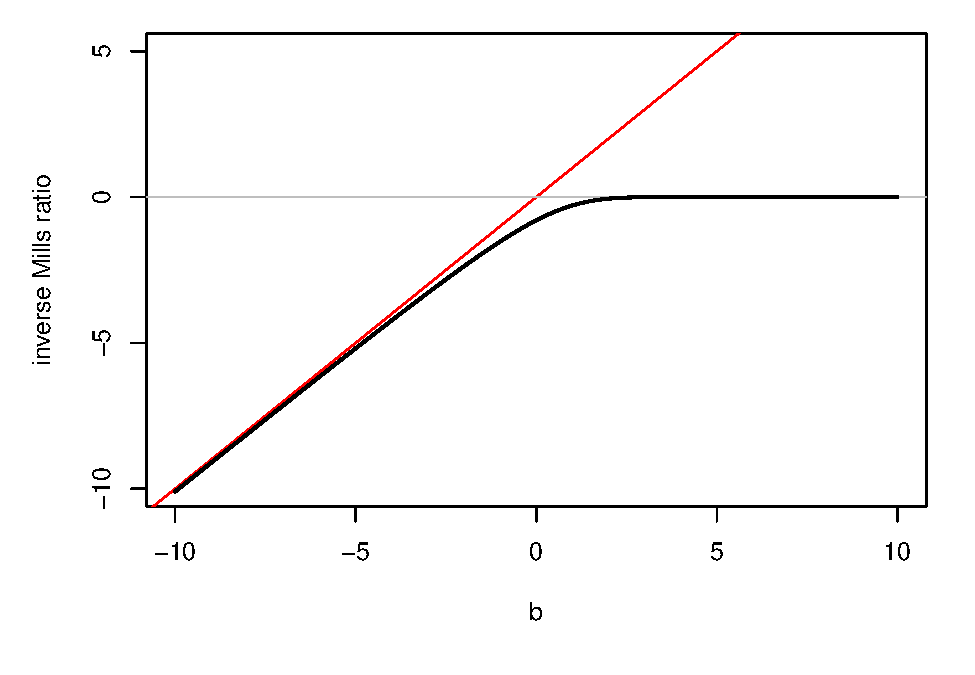
\includegraphics{AdvECTS_files/figure-latex/inverseMills-1} 

}

\caption{$\mathbb{E}(X|X<b)$ as a function of $b$ when $X\sim \mathcal{N}(0,1)$ (in black).}\label{fig:inverseMills}
\end{figure}

\begin{proposition}[p.d.f. of a multivariate Gaussian variable]
\protect\hypertarget{prp:pdfMultivarGaussian}{}\label{prp:pdfMultivarGaussian}If \(Y \sim \mathcal{N}(\mu,\Omega)\) and if \(Y\) is a \(n\)-dimensional vector, then the density function of \(Y\) is:
\[
\frac{1}{(2 \pi)^{n/2}|\Omega|^{1/2}}\exp\left[-\frac{1}{2}\left(Y-\mu\right)'\Omega^{-1}\left(Y-\mu\right)\right].
\]
\end{proposition}

\hypertarget{proofs}{%
\section{Proofs}\label{proofs}}

\hypertarget{MLEproperties}{%
\subsection{Proof of Proposition \ref{prp:MLEproperties}}\label{MLEproperties}}

\begin{proof}
Assumptions (i) and (ii) (in the set of Assumptions \ref{hyp:MLEregularity}) imply that \(\boldsymbol\theta_{MLE}\) exists (\(=\mbox{argmax}_\theta (1/n)\log \mathcal{L}(\boldsymbol\theta;\mathbf{y})\)).

\((1/n)\log \mathcal{L}(\boldsymbol\theta;\mathbf{y})\) can be interpreted as the sample mean of the r.v. \(\log f(Y_i;\boldsymbol\theta)\) that are i.i.d. Therefore \((1/n)\log \mathcal{L}(\boldsymbol\theta;\mathbf{y})\) converges to \(\mathbb{E}_{\boldsymbol\theta_0}(\log f(Y;\boldsymbol\theta))\) -- which exists (Assumption iv).

Because the latter convergence is uniform (Assumption v), the solution \(\boldsymbol\theta_{MLE}\) almost surely converges to the solution to the limit problem:
\[
\mbox{argmax}_\theta \mathbb{E}_{\boldsymbol\theta_0}(\log f(Y;\boldsymbol\theta)) = \mbox{argmax}_\theta \int_{\mathcal{Y}} \log f(y;\boldsymbol\theta)f(y;\boldsymbol\theta_0) dy.
\]

Properties of the Kullback information measure (see Prop. \ref{prp:Kullback}), together with the identifiability assumption (ii) implies that the solution to the limit problem is unique and equal to \(\boldsymbol\theta_0\).

Consider a r.v. sequence \(\boldsymbol\theta\) that converges to \(\boldsymbol\theta_0\). The Taylor expansion of the score in a neighborood of \(\boldsymbol\theta_0\) yields to:
\[
\frac{\partial \log \mathcal{L}(\boldsymbol\theta;\mathbf{y})}{\partial \boldsymbol\theta} = \frac{\partial \log \mathcal{L}(\boldsymbol\theta_0;\mathbf{y})}{\partial \boldsymbol\theta} + \frac{\partial^2 \log \mathcal{L}(\boldsymbol\theta_0;\mathbf{y})}{\partial \boldsymbol\theta \partial \boldsymbol\theta'}(\boldsymbol\theta - \boldsymbol\theta_0) + o_p(\boldsymbol\theta - \boldsymbol\theta_0)
\]

\(\boldsymbol\theta_{MLE}\) converges to \(\boldsymbol\theta_0\) and satisfies the likelihood equation \(\frac{\partial \log \mathcal{L}(\boldsymbol\theta;\mathbf{y})}{\partial \boldsymbol\theta} = \mathbf{0}\). Therefore:
\[
\frac{\partial \log \mathcal{L}(\boldsymbol\theta_0;\mathbf{y})}{\partial \boldsymbol\theta} \approx - \frac{\partial^2 \log \mathcal{L}(\boldsymbol\theta_0;\mathbf{y})}{\partial \boldsymbol\theta \partial \boldsymbol\theta'}(\boldsymbol\theta_{MLE} - \boldsymbol\theta_0),
\]
or equivalently:
\[
\frac{1}{\sqrt{n}} \frac{\partial \log \mathcal{L}(\boldsymbol\theta_0;\mathbf{y})}{\partial \boldsymbol\theta} \approx
\left(- \frac{1}{n} \sum_{i=1}^n \frac{\partial^2 \log f(y_i;\boldsymbol\theta_0)}{\partial \boldsymbol\theta \partial \boldsymbol\theta'} \right)\sqrt{n}(\boldsymbol\theta_{MLE} - \boldsymbol\theta_0),
\]

By the law of large numbers, we have: \(\left(- \frac{1}{n} \sum_{i=1}^n \frac{\partial^2 \log f(y_i;\boldsymbol\theta_0)}{\partial \boldsymbol\theta \partial \boldsymbol\theta'} \right) \overset{}\rightarrow \frac{1}{n} \mathbf{I}(\boldsymbol\theta_0) = \mathcal{I}_Y(\boldsymbol\theta_0)\).

Besides, we have:
\begin{eqnarray*}
\frac{1}{\sqrt{n}} \frac{\partial \log \mathcal{L}(\boldsymbol\theta_0;\mathbf{y})}{\partial \boldsymbol\theta} &=& \sqrt{n} \left( \frac{1}{n} \sum_i \frac{\partial \log f(y_i;\boldsymbol\theta_0)}{\partial \boldsymbol\theta} \right) \\
&=& \sqrt{n} \left( \frac{1}{n} \sum_i \left\{ \frac{\partial \log f(y_i;\boldsymbol\theta_0)}{\partial \boldsymbol\theta} - \mathbb{E}_{\boldsymbol\theta_0} \frac{\partial \log f(Y_i;\boldsymbol\theta_0)}{\partial \boldsymbol\theta} \right\} \right)
\end{eqnarray*}
which converges to \(\mathcal{N}(0,\mathcal{I}_Y(\boldsymbol\theta_0))\) by the CLT.

Collecting the preceding results leads to (b). The fact that \(\boldsymbol\theta_{MLE}\) achieves the FDCR bound proves (c).
\end{proof}

\hypertarget{Walddistri}{%
\subsection{Proof of Proposition \ref{prp:Walddistri}}\label{Walddistri}}

\begin{proof}
We have \(\sqrt{n}(\hat{\boldsymbol\theta}_{n} - \boldsymbol\theta_{0}) \overset{d}{\rightarrow} \mathcal{N}(0,\mathcal{I}(\boldsymbol\theta_0)^{-1})\) (Eq. \ref(eq:normMLE)). A Taylor expansion around \(\boldsymbol\theta_0\) yields to:
\begin{equation}
\sqrt{n}(h(\hat{\boldsymbol\theta}_{n}) - h(\boldsymbol\theta_{0})) \overset{d}{\rightarrow} \mathcal{N}\left(0,\frac{\partial h(\boldsymbol\theta_{0})}{\partial \boldsymbol\theta'}\mathcal{I}(\boldsymbol\theta_0)^{-1}\frac{\partial h(\boldsymbol\theta_{0})'}{\partial \boldsymbol\theta}\right). \label{eq:XXX}
\end{equation}
Under \(H_0\), \(h(\boldsymbol\theta_{0})=0\) therefore:
\begin{equation}
\sqrt{n} h(\hat{\boldsymbol\theta}_{n}) \overset{d}{\rightarrow} \mathcal{N}\left(0,\frac{\partial h(\boldsymbol\theta_{0})}{\partial \boldsymbol\theta'}\mathcal{I}(\boldsymbol\theta_0)^{-1}\frac{\partial h(\boldsymbol\theta_{0})'}{\partial \boldsymbol\theta}\right). \label{eq:lm10}
\end{equation}
Hence
\[
\sqrt{n} \left(
\frac{\partial h(\boldsymbol\theta_{0})}{\partial \boldsymbol\theta'}\mathcal{I}(\boldsymbol\theta_0)^{-1}\frac{\partial h(\boldsymbol\theta_{0})'}{\partial \boldsymbol\theta}
\right)^{-1/2} h(\hat{\boldsymbol\theta}_{n}) \overset{d}{\rightarrow} \mathcal{N}\left(0,Id\right).
\]
Taking the quadratic form, we obtain:
\[
n h(\hat{\boldsymbol\theta}_{n})'  \left(
\frac{\partial h(\boldsymbol\theta_{0})}{\partial \boldsymbol\theta'}\mathcal{I}(\boldsymbol\theta_0)^{-1}\frac{\partial h(\boldsymbol\theta_{0})'}{\partial \boldsymbol\theta}
\right)^{-1} h(\hat{\boldsymbol\theta}_{n}) \overset{d}{\rightarrow} \chi^2(r).
\]

The fact that the test has asymptotic level \(\alpha\) directly stems from what precedes. \textbf{Consistency of the test}: Consider \(\theta_0 \in \Theta\). Because the MLE is consistent, \(h(\hat{\boldsymbol\theta}_{n})\) converges to \(h(\boldsymbol\theta_0) \ne 0\). Eq. \eqref{eq:XXX} is still valid. It implies that \(\xi^W_n\) converges to \(+\infty\) and therefore that \(\mathbb{P}_{\boldsymbol\theta}(\xi^W_n \ge \chi^2_{1-\alpha}(r)) \rightarrow 1\).
\end{proof}

\hypertarget{LMdistri}{%
\subsection{Proof of Proposition \ref{prp:LMdistri}}\label{LMdistri}}

\begin{proof}
Notations: ``\(\approx\)'' means ``equal up to a term that converges to 0 in probability''. We are under \(H_0\). \(\hat{\boldsymbol\theta}^0\) is the constrained ML estimator; \(\hat{\boldsymbol\theta}\) denotes the unconstrained one.

We combine the two Taylor expansion: \(h(\hat{\boldsymbol\theta}_n) \approx \dfrac{\partial h(\boldsymbol\theta_0)}{\partial \boldsymbol\theta'}(\hat{\boldsymbol\theta}_n - \boldsymbol\theta_0)\) and \(h(\hat{\boldsymbol\theta}_n^0) \approx \dfrac{\partial h(\boldsymbol\theta_0)}{\partial \boldsymbol\theta'}(\hat{\boldsymbol\theta}_n^0 - \boldsymbol\theta_0)\) and we use \(h(\hat{\boldsymbol\theta}_n^0)=0\) (by definition) to get:
\begin{equation}
\sqrt{n}h(\hat{\boldsymbol\theta}_n) \approx \dfrac{\partial h(\boldsymbol\theta_0)}{\partial \boldsymbol\theta'}\sqrt{n}(\hat{\boldsymbol\theta}_n - \hat{\boldsymbol\theta}^0_n). \label{eq:lm1}
\end{equation}
Besides, we have (using the definition of the information matrix):
\begin{equation}
\frac{1}{\sqrt{n}}\frac{\partial \log \mathcal{L}(\hat{\boldsymbol\theta}^0_n;\mathbf{y})}{\partial \boldsymbol\theta} \approx
\frac{1}{\sqrt{n}}\frac{\partial \log \mathcal{L}(\boldsymbol\theta_0;\mathbf{y})}{\partial \boldsymbol\theta} - \mathcal{I}(\boldsymbol\theta_0)\sqrt{n}(\hat{\boldsymbol\theta}^0_n-\boldsymbol\theta_0) \label{eq:lm29}
\end{equation}
and:
\begin{equation}
0=\frac{1}{\sqrt{n}}\frac{\partial \log \mathcal{L}(\hat{\boldsymbol\theta}_n;\mathbf{y})}{\partial \boldsymbol\theta} \approx
\frac{1}{\sqrt{n}}\frac{\partial \log \mathcal{L}(\boldsymbol\theta_0;\mathbf{y})}{\partial \boldsymbol\theta} - \mathcal{I}(\boldsymbol\theta_0)\sqrt{n}(\hat{\boldsymbol\theta}_n-\boldsymbol\theta_0).\label{eq:lm30}
\end{equation}
Taking the difference and multiplying by \(\mathcal{I}(\boldsymbol\theta_0)^{-1}\):
\begin{equation}
\sqrt{n}(\hat{\boldsymbol\theta}_n-\hat{\boldsymbol\theta}_n^0) \approx
\mathcal{I}(\boldsymbol\theta_0)^{-1}\frac{1}{\sqrt{n}}\frac{\partial \log \mathcal{L}(\hat{\boldsymbol\theta}^0_n;\mathbf{y})}{\partial \boldsymbol\theta}
\mathcal{I}(\boldsymbol\theta_0).\label{eq:lm2}
\end{equation}
Eqs. \eqref{eq:lm1} and \eqref{eq:lm2} yield to:
\begin{equation}
\sqrt{n}h(\hat{\boldsymbol\theta}_n) \approx \dfrac{\partial h(\boldsymbol\theta_0)}{\partial \boldsymbol\theta'} \mathcal{I}(\boldsymbol\theta_0)^{-1}\frac{1}{\sqrt{n}}\frac{\partial \log \mathcal{L}(\hat{\boldsymbol\theta}^0_n;\mathbf{y})}{\partial \boldsymbol\theta}.\label{eq:lm3}
\end{equation}

Recall that \(\hat{\boldsymbol\theta}^0_n\) is the MLE of \(\boldsymbol\theta_0\) under the constraint \(h(\boldsymbol\theta)=0\). The vector of Lagrange multipliers \(\hat\lambda_n\) associated to this program satisfies:
\begin{equation}
\frac{\partial \log \mathcal{L}(\hat{\boldsymbol\theta}^0_n;\mathbf{y})}{\partial \boldsymbol\theta}+ \frac{\partial h'(\hat{\boldsymbol\theta}^0_n;\mathbf{y})}{\partial \boldsymbol\theta}\hat\lambda_n = 0.\label{eq:multiplier}
\end{equation}
Substituting the latter equation in Eq. \eqref{eq:lm3} gives:
\[
\sqrt{n}h(\hat{\boldsymbol\theta}_n) \approx
- \dfrac{\partial h(\boldsymbol\theta_0)}{\partial \boldsymbol\theta'} \mathcal{I}(\boldsymbol\theta_0)^{-1}
\frac{\partial h'(\hat{\boldsymbol\theta}^0_n;\mathbf{y})}{\partial \boldsymbol\theta} \frac{\hat\lambda_n}{\sqrt{n}} \approx
- \dfrac{\partial h(\boldsymbol\theta_0)}{\partial \boldsymbol\theta'} \mathcal{I}(\boldsymbol\theta_0)^{-1}
\frac{\partial h'(\boldsymbol\theta_0;\mathbf{y})}{\partial \boldsymbol\theta} \frac{\hat\lambda_n}{\sqrt{n}}
\]
which yields:
\begin{equation}
\frac{\hat\lambda_n}{\sqrt{n}} \approx - \left(
\dfrac{\partial h(\boldsymbol\theta_0)}{\partial \boldsymbol\theta'} \mathcal{I}(\boldsymbol\theta_0)^{-1}
\frac{\partial h'(\boldsymbol\theta_0;\mathbf{y})}{\partial \boldsymbol\theta}
\right)^{-1}
\sqrt{n}h(\hat{\boldsymbol\theta}_n).\label{eq:lm20}
\end{equation}
It follows, from Eq. \eqref{eq:lm10}, that:
\[
\frac{\hat\lambda_n}{\sqrt{n}} \overset{d}{\rightarrow} \mathcal{N}\left(0,\left(
\dfrac{\partial h(\boldsymbol\theta_0)}{\partial \boldsymbol\theta'} \mathcal{I}(\boldsymbol\theta_0)^{-1}
\frac{\partial h'(\boldsymbol\theta_0;\mathbf{y})}{\partial \boldsymbol\theta}
\right)^{-1}\right).
\]
Taking the quadratic form of the last equation gives:
\[
\frac{1}{n}\hat\lambda_n' \dfrac{\partial h(\hat{\boldsymbol\theta}^0_n)}{\partial \boldsymbol\theta'} \mathcal{I}(\hat{\boldsymbol\theta}^0_n)^{-1}
\frac{\partial h'(\hat{\boldsymbol\theta}^0_n;\mathbf{y})}{\partial \boldsymbol\theta} \hat\lambda_n \overset{d}{\rightarrow} \chi^2(r).
\]
Using Eq. \eqref{eq:multiplier}, it appears that the left-hand side term of the last equation is \(\xi^{LM}\) as defined in Eq. \eqref{eq:xiLM}. Consistency: see Remark 17.3 in \citet{gourieroux_monfort_1995}.
\end{proof}

\hypertarget{equivWaldLM}{%
\subsection{Proof of Proposition \ref{prp:equivWaldLM}}\label{equivWaldLM}}

\begin{proof}
We have (using Eq. \ref(eq:multiplier)):
\[
\xi^{LM}_n = \frac{1}{n}\hat\lambda_n' \dfrac{\partial h(\hat{\boldsymbol\theta}^0_n)}{\partial \boldsymbol\theta'} \mathcal{I}(\hat{\boldsymbol\theta}^0_n)^{-1}
\frac{\partial h'(\hat{\boldsymbol\theta}^0_n;\mathbf{y})}{\partial \boldsymbol\theta} \hat\lambda_n.
\]
Since, under \(H_0\), \(\hat{\boldsymbol\theta}_n^0\approx\hat{\boldsymbol\theta}_n \approx {\boldsymbol\theta}_0\), Eq. \eqref{eq:lm20} therefore implies that:
\[
\xi^{LM} \approx n h(\hat{\boldsymbol\theta}_n)' \left(
\dfrac{\partial h(\hat{\boldsymbol\theta}_n)}{\partial \boldsymbol\theta'} \mathcal{I}(\hat{\boldsymbol\theta}_n)^{-1}
\frac{\partial h'(\hat{\boldsymbol\theta}_n;\mathbf{y})}{\partial \boldsymbol\theta}
\right)^{-1}
h(\hat{\boldsymbol\theta}_n) = \xi^{W},
\]
which gives the result.
\end{proof}

\hypertarget{equivLRLM}{%
\subsection{Proof of Proposition \ref{prp:equivLRLM}}\label{equivLRLM}}

\begin{proof}
The second-order taylor expansions of \(\log \mathcal{L}(\hat{\boldsymbol\theta}^0_n,\mathbf{y})\) and \(\log \mathcal{L}(\hat{\boldsymbol\theta}_n,\mathbf{y})\) are:
\begin{eqnarray*}
\log \mathcal{L}(\hat{\boldsymbol\theta}_n,\mathbf{y}) &\approx& \log \mathcal{L}(\boldsymbol\theta_0,\mathbf{y})
+ \frac{\partial \log \mathcal{L}(\boldsymbol\theta_0,\mathbf{y})}{\partial \boldsymbol\theta'}(\hat{\boldsymbol\theta}_n-\boldsymbol\theta_0)
- \frac{n}{2} (\hat{\boldsymbol\theta}_n-\boldsymbol\theta_0)' \mathcal{I}(\boldsymbol\theta_0) (\hat{\boldsymbol\theta}_n-\boldsymbol\theta_0)\\
\log \mathcal{L}(\hat{\boldsymbol\theta}^0_n,\mathbf{y}) &\approx& \log \mathcal{L}(\boldsymbol\theta_0,\mathbf{y})
+ \frac{\partial \log \mathcal{L}(\boldsymbol\theta_0,\mathbf{y})}{\partial \boldsymbol\theta'}(\hat{\boldsymbol\theta}^0_n-\boldsymbol\theta_0)
- \frac{n}{2} (\hat{\boldsymbol\theta}^0_n-\boldsymbol\theta_0)' \mathcal{I}(\boldsymbol\theta_0) (\hat{\boldsymbol\theta}^0_n-\boldsymbol\theta_0).
\end{eqnarray*}
Taking the difference, we obtain:
\[
\xi_n^{LR} \approx 2\frac{\partial \log \mathcal{L}(\boldsymbol\theta_0,\mathbf{y})}{\partial \boldsymbol\theta'}
(\hat{\boldsymbol\theta}_n-\hat{\boldsymbol\theta}^0_n) + n (\hat{\boldsymbol\theta}^0_n-\boldsymbol\theta_0)' \mathcal{I}(\boldsymbol\theta_0) (\hat{\boldsymbol\theta}^0_n-\boldsymbol\theta_0) - n (\hat{\boldsymbol\theta}_n-\boldsymbol\theta_0)' \mathcal{I}(\boldsymbol\theta_0) (\hat{\boldsymbol\theta}_n-\boldsymbol\theta_0).
\]
Using \(\dfrac{1}{\sqrt{n}}\frac{\partial \log \mathcal{L}(\boldsymbol\theta_0;\mathbf{y})}{\partial \boldsymbol\theta} \approx \mathcal{I}(\boldsymbol\theta_0)\sqrt{n}(\hat{\boldsymbol\theta}_n-\boldsymbol\theta_0)\) (Eq. \eqref{eq:lm30}), we have:
\[
\xi_n^{LR} \approx
2n(\hat{\boldsymbol\theta}_n-\boldsymbol\theta_0)'\mathcal{I}(\boldsymbol\theta_0)
(\hat{\boldsymbol\theta}_n-\hat{\boldsymbol\theta}^0_n)
+ n (\hat{\boldsymbol\theta}^0_n-\boldsymbol\theta_0)' \mathcal{I}(\boldsymbol\theta_0) (\hat{\boldsymbol\theta}^0_n-\boldsymbol\theta_0) - n (\hat{\boldsymbol\theta}_n-\boldsymbol\theta_0)' \mathcal{I}(\boldsymbol\theta_0) (\hat{\boldsymbol\theta}_n-\boldsymbol\theta_0).
\]
In the second of the three terms in the sum, we replace \((\hat{\boldsymbol\theta}^0_n-\boldsymbol\theta_0)\) by \((\hat{\boldsymbol\theta}^0_n-\hat{\boldsymbol\theta}_n+\hat{\boldsymbol\theta}_n-\boldsymbol\theta_0)\) and we develop the associated product. This leads to:
\begin{equation}
\xi_n^{LR} \approx n (\hat{\boldsymbol\theta}^0_n-\hat{\boldsymbol\theta}_n)' \mathcal{I}(\boldsymbol\theta_0)^{-1} (\hat{\boldsymbol\theta}^0_n-\hat{\boldsymbol\theta}_n). \label{eq:lr10}
\end{equation}
The difference between Eqs. \eqref{eq:lm29} and \eqref{eq:lm30} implies:
\[
\frac{1}{\sqrt{n}}\frac{\partial \log \mathcal{L}(\hat{\boldsymbol\theta}^0_n;\mathbf{y})}{\partial \boldsymbol\theta} \approx
\mathcal{I}(\boldsymbol\theta_0)\sqrt{n}(\hat{\boldsymbol\theta}_n-\hat{\boldsymbol\theta}^0_n),
\]
which, associated to Eq. @\ref(eq:lr10), gives:
\[
\xi_n^{LR} \approx \frac{1}{n} \frac{\partial \log \mathcal{L}(\hat{\boldsymbol\theta}^0_n;\mathbf{y})}{\partial \boldsymbol\theta'} \mathcal{I}(\boldsymbol\theta_0)^{-1} \frac{\partial \log \mathcal{L}(\hat{\boldsymbol\theta}^0_n;\mathbf{y})}{\partial \boldsymbol\theta} \approx \xi_n^{LM}.
\]
Hence \(\xi_n^{LR}\) has the same asymptotic distribution as \(\xi_n^{LM}\).

Let's show that the test is consistent. For this, note that:
\[
\frac{\log \mathcal{L}(\hat{\boldsymbol\theta},\mathbf{y}) - \log \mathcal{L}(\hat{\boldsymbol\theta}^0,\mathbf{y})}{n} = \frac{1}{n} \sum_{i=1}^n[\log f(y_i;\hat{\boldsymbol\theta}_n) - \log f(y_i;\hat{\boldsymbol\theta}_n^0)] \rightarrow \mathbb{E}_0[\log f(Y;\boldsymbol\theta_0) - \log f(Y;\boldsymbol\theta_\infty)],
\]
where \(\boldsymbol\theta_\infty\), the pseudo true value, is such that \(h(\boldsymbol\theta_\infty) \ne 0\) (by definition of \(H_1\)). From the Kullback inequality and the asymptotic identifiability of \(\boldsymbol\theta_0\), it follows that \(\mathbb{E}_0[\log f(Y;\boldsymbol\theta_0) - \log f(Y;\boldsymbol\theta_\infty)] >0\). Therefore \(\xi_n^{LR} \rightarrow + \infty\) under \(H_1\).
\end{proof}

\hypertarget{proofTVTCL}{%
\subsection{Proof of Eq. \eqref{eq:TCL2}}\label{proofTVTCL}}

\begin{proof}
We have:
\begin{eqnarray*}
&&T\mathbb{E}\left[(\bar{y}_T - \mu)^2\right]\\
&=& T\mathbb{E}\left[\left(\frac{1}{T}\sum_{t=1}^T(y_t - \mu)\right)^2\right] = \frac{1}{T} \mathbb{E}\left[\sum_{t=1}^T(y_t - \mu)^2+2\sum_{s<t\le T}(y_t - \mu)(y_s - \mu)\right]\\
&=& \gamma_0 +\frac{2}{T}\left(\sum_{t=2}^{T}\mathbb{E}\left[(y_t - \mu)(y_{t-1} - \mu)\right]\right) +\frac{2}{T}\left(\sum_{t=3}^{T}\mathbb{E}\left[(y_t - \mu)(y_{t-2} - \mu)\right]\right) + \dots \\
&&+ \frac{2}{T}\left(\sum_{t=T-1}^{T}\mathbb{E}\left[(y_t - \mu)(y_{t-(T-2)} - \mu)\right]\right) + \frac{2}{T}\mathbb{E}\left[(y_t - \mu)(y_{t-(T-1)} - \mu)\right]\\
&=&  \gamma_0 + 2 \frac{T-1}{T}\gamma_1 + \dots + 2 \frac{1}{T}\gamma_{T-1} .
\end{eqnarray*}
Therefore:
\begin{eqnarray*}
T\mathbb{E}\left[(\bar{y}_T - \mu)^2\right] - \sum_{j=-\infty}^{+\infty} \gamma_j &=& - 2\frac{1}{T}\gamma_1 - 2\frac{2}{T}\gamma_2 - \dots - 2\frac{T-1}{T}\gamma_{T-1} - 2\gamma_T - 2 \gamma_{T+1} + \dots
\end{eqnarray*}
And then:
\[
\left|T\mathbb{E}\left[(\bar{y}_T - \mu)^2\right] - \sum_{j=-\infty}^{+\infty} \gamma_j\right| \le 2\frac{1}{T}|\gamma_1| + 2\frac{2}{T}|\gamma_2| + \dots + 2\frac{T-1}{T}|\gamma_{T-1}| + 2|\gamma_T| + 2 |\gamma_{T+1}| + \dots
\]

For any \(q \le T\), we have:
\begin{eqnarray*}
\left|T\mathbb{E}\left[(\bar{y}_T - \mu)^2\right] - \sum_{j=-\infty}^{+\infty} \gamma_j\right| &\le& 2\frac{1}{T}|\gamma_1| + 2\frac{2}{T}|\gamma_2| + \dots + 2\frac{q-1}{T}|\gamma_{q-1}| +2\frac{q}{T}|\gamma_q| +\\
&&2\frac{q+1}{T}|\gamma_{q+1}| + \dots  + 2\frac{T-1}{T}|\gamma_{T-1}| + 2|\gamma_T| + 2 |\gamma_{T+1}| + \dots\\
&\le& \frac{2}{T}\left(|\gamma_1| + 2|\gamma_2| + \dots + (q-1)|\gamma_{q-1}| +q|\gamma_q|\right) +\\
&&2|\gamma_{q+1}| + \dots  + 2|\gamma_{T-1}| + 2|\gamma_T| + 2 |\gamma_{T+1}| + \dots
\end{eqnarray*}

Consider \(\varepsilon > 0\). The fact that the autocovariances are absolutely summable implies that there exists \(q_0\) such that (Cauchy criterion, Theorem \ref{thm:cauchycritstatic}):
\[
2|\gamma_{q_0+1}|+2|\gamma_{q_0+2}|+2|\gamma_{q_0+3}|+\dots < \varepsilon/2.
\]
Then, if \(T > q_0\), it comes that:
\[
\left|T \mathbb{E}\left[(\bar{y}_T - \mu)^2\right] - \sum_{j=-\infty}^{+\infty} \gamma_j\right|\le \frac{2}{T}\left(|\gamma_1| + 2|\gamma_2| + \dots + (q_0-1)|\gamma_{q_0-1}| +q_0|\gamma_{q_0}|\right) + \varepsilon/2.
\]
If \(T \ge 2\left(|\gamma_1| + 2|\gamma_2| + \dots + (q_0-1)|\gamma_{q_0-1}| +q_0|\gamma_{q_0}|\right)/(\varepsilon/2)\) (\(= f(q_0)\), say) then
\[
\frac{2}{T}\left(|\gamma_1| + 2|\gamma_2| + \dots + (q_0-1)|\gamma_{q_0-1}| +q_0|\gamma_{q_0}|\right) \le \varepsilon/2.
\]
Then, if \(T>f(q_0)\) and \(T>q_0\), i.e.~if \(T>\max(f(q_0),q_0)\), we have:
\[
\left|T \mathbb{E}\left[(\bar{y}_T - \mu)^2\right] - \sum_{j=-\infty}^{+\infty} \gamma_j\right|\le \varepsilon.
\]
\end{proof}

\hypertarget{smallestMSE}{%
\subsection{Proof of Proposition \ref{prp:smallestMSE}}\label{smallestMSE}}

\begin{proof}
We have:
\begin{eqnarray}
\mathbb{E}([y_{t+1} - y^*_{t+1}]^2) &=& \mathbb{E}\left([\color{blue}{\{y_{t+1} - \mathbb{E}(y_{t+1}|x_t)\}} + \color{red}{\{\mathbb{E}(y_{t+1}|x_t)  - y^*_{t+1}\}}]^2\right)\nonumber\\
&=&  \mathbb{E}\left(\color{blue}{[y_{t+1} - \mathbb{E}(y_{t+1}|x_t)]}^2\right) + \mathbb{E}\left(\color{red}{[\mathbb{E}(y_{t+1}|x_t)  - y^*_{t+1}]}^2\right)\nonumber\\
&& + 2\mathbb{E}\left( \color{blue}{[y_{t+1} - \mathbb{E}(y_{t+1}|x_t)]}\color{red}{ [\mathbb{E}(y_{t+1}|x_t)  - y^*_{t+1}]}\right). \label{eq:1}
\end{eqnarray}
Let us focus on the last term. We have:
\begin{eqnarray*}
&&\mathbb{E}\left(\color{blue}{[y_{t+1} - \mathbb{E}(y_{t+1}|x_t)]}\color{red}{ [\mathbb{E}(y_{t+1}|x_t)  - y^*_{t+1}]}\right)\\
&=& \mathbb{E}( \mathbb{E}( \color{blue}{[y_{t+1} - \mathbb{E}(y_{t+1}|x_t)]}\color{red}{ \underbrace{[\mathbb{E}(y_{t+1}|x_t)  - y^*_{t+1}]}_{\mbox{function of $x_t$}}}|x_t))\\
&=& \mathbb{E}( \color{red}{ [\mathbb{E}(y_{t+1}|x_t)  - y^*_{t+1}]} \mathbb{E}( \color{blue}{[y_{t+1} - \mathbb{E}(y_{t+1}|x_t)]}|x_t))\\
&=& \mathbb{E}( \color{red}{ [\mathbb{E}(y_{t+1}|x_t)  - y^*_{t+1}]} \color{blue}{\underbrace{[\mathbb{E}(y_{t+1}|x_t) - \mathbb{E}(y_{t+1}|x_t)]}_{=0}})=0.
\end{eqnarray*}

Therefore, Eq. \eqref{eq:1} becomes:
\begin{eqnarray*}
&&\mathbb{E}([y_{t+1} - y^*_{t+1}]^2) \\
&=&  \underbrace{\mathbb{E}\left(\color{blue}{[y_{t+1} - \mathbb{E}(y_{t+1}|x_t)]}^2\right)}_{\mbox{$\ge 0$ and does not depend on $y^*_{t+1}$}} + \underbrace{\mathbb{E}\left(\color{red}{[\mathbb{E}(y_{t+1}|x_t)  - y^*_{t+1}]}^2\right)}_{\mbox{$\ge 0$ and depends on $y^*_{t+1}$}}.
\end{eqnarray*}
This implies that \(\mathbb{E}([y_{t+1} - y^*_{t+1}]^2)\) is always larger than \(\color{blue}{\mathbb{E}([y_{t+1} - \mathbb{E}(y_{t+1}|x_t)]^2)}\), and is therefore minimized if the second term is equal to zero, that is if \(\mathbb{E}(y_{t+1}|x_t) = y^*_{t+1}\).
\end{proof}

\hypertarget{estimVARGaussian}{%
\subsection{Proof of Proposition \ref{prp:estimVARGaussian}}\label{estimVARGaussian}}

\begin{proof}
Using Proposition \ref{prp:multivarG} (in Appendix \ref{XXX}), we obtain that, conditionally on \(x_1\), the log-likelihood is given by
\begin{eqnarray*}
\log\mathcal{L}(Y_{T};\theta) & = & -(Tn/2)\log(2\pi)+(T/2)\log\left|\Omega^{-1}\right|\\
&  & -\frac{1}{2}\sum_{t=1}^{T}\left[\left(y_{t}-\Pi'x_{t}\right)'\Omega^{-1}\left(y_{t}-\Pi'x_{t}\right)\right].
\end{eqnarray*}
Let's rewrite the last term of the log-likelihood:
\begin{eqnarray*}
\sum_{t=1}^{T}\left[\left(y_{t}-\Pi'x_{t}\right)'\Omega^{-1}\left(y_{t}-\Pi'x_{t}\right)\right] & =\\
\sum_{t=1}^{T}\left[\left(y_{t}-\hat{\Pi}'x_{t}+\hat{\Pi}'x_{t}-\Pi'x_{t}\right)'\Omega^{-1}\left(y_{t}-\hat{\Pi}'x_{t}+\hat{\Pi}'x_{t}-\Pi'x_{t}\right)\right] & =\\
\sum_{t=1}^{T}\left[\left(\hat{\varepsilon}_{t}+(\hat{\Pi}-\Pi)'x_{t}\right)'\Omega^{-1}\left(\hat{\varepsilon}_{t}+(\hat{\Pi}-\Pi)'x_{t}\right)\right],
\end{eqnarray*}
where the \(j^{th}\) element of the \((n\times1)\) vector \(\hat{\varepsilon}_{t}\) is the sample residual, for observation \(t\), from an OLS regression of \(y_{j,t}\) on \(x_{t}\). Expanding the previous equation, we get:
\begin{eqnarray*}
&&\sum_{t=1}^{T}\left[\left(y_{t}-\Pi'x_{t}\right)'\Omega^{-1}\left(y_{t}-\Pi'x_{t}\right)\right]  = \sum_{t=1}^{T}\hat{\varepsilon}_{t}'\Omega^{-1}\hat{\varepsilon}_{t}\\
&&+2\sum_{t=1}^{T}\hat{\varepsilon}_{t}'\Omega^{-1}(\hat{\Pi}-\Pi)'x_{t}+\sum_{t=1}^{T}x'_{t}(\hat{\Pi}-\Pi)\Omega^{-1}(\hat{\Pi}-\Pi)'x_{t}.
\end{eqnarray*}
Let's apply the trace operator on the second term (that is a scalar):
\begin{eqnarray*}
\sum_{t=1}^{T}\hat{\varepsilon}_{t}'\Omega^{-1}(\hat{\Pi}-\Pi)'x_{t} & = & Tr\left(\sum_{t=1}^{T}\hat{\varepsilon}_{t}'\Omega^{-1}(\hat{\Pi}-\Pi)'x_{t}\right)\\
=  Tr\left(\sum_{t=1}^{T}\Omega^{-1}(\hat{\Pi}-\Pi)'x_{t}\hat{\varepsilon}_{t}'\right) & = & Tr\left(\Omega^{-1}(\hat{\Pi}-\Pi)'\sum_{t=1}^{T}x_{t}\hat{\varepsilon}_{t}'\right).
\end{eqnarray*}
Given that, by construction (property of OLS estimates), the sample residuals are orthogonal to the explanatory variables, this term is zero. Introducing \(\tilde{x}_{t}=(\hat{\Pi}-\Pi)'x_{t}\), we have
\begin{eqnarray*}
\sum_{t=1}^{T}\left[\left(y_{t}-\Pi'x_{t}\right)'\Omega^{-1}\left(y_{t}-\Pi'x_{t}\right)\right] =\sum_{t=1}^{T}\hat{\varepsilon}_{t}'\Omega^{-1}\hat{\varepsilon}_{t}+\sum_{t=1}^{T}\tilde{x}'_{t}\Omega^{-1}\tilde{x}_{t}.
\end{eqnarray*}
Since \(\Omega\) is a positive definite matrix, \(\Omega^{-1}\) is as well. Consequently, the smallest value that the last term can take is obtained for \(\tilde{x}_{t}=0\), i.e.~when \(\Pi=\hat{\Pi}.\)

The MLE of \(\Omega\) is the matrix \(\hat{\Omega}\) that maximizes \(\Omega\overset{\ell}{\rightarrow}L(Y_{T};\hat{\Pi},\Omega)\). We have:
\begin{eqnarray*}
\log\mathcal{L}(Y_{T};\hat{\Pi},\Omega) & = & -(Tn/2)\log(2\pi)+(T/2)\log\left|\Omega^{-1}\right| -\frac{1}{2}\sum_{t=1}^{T}\left[\hat{\varepsilon}_{t}'\Omega^{-1}\hat{\varepsilon}_{t}\right].
\end{eqnarray*}

Matrix \(\hat{\Omega}\) is a symmetric positive definite. It is easily checked that the (unrestricted) matrix that maximizes the latter expression is symmetric positive definite matrix. Indeed:
\[
\frac{\partial \log\mathcal{L}(Y_{T};\hat{\Pi},\Omega)}{\partial\Omega}=\frac{T}{2}\Omega'-\frac{1}{2}\sum_{t=1}^{T}\hat{\varepsilon}_{t}\hat{\varepsilon}'_{t}\Rightarrow\hat{\Omega}'=\frac{1}{T}\sum_{t=1}^{T}\hat{\varepsilon}_{t}\hat{\varepsilon}'_{t},
\]
which leads to the result.
\end{proof}

\hypertarget{OLSVAR}{%
\subsection{Proof of Proposition \ref{prp:OLSVAR}}\label{OLSVAR}}

\begin{proof}
Let us drop the \(i\) subscript. Rearranging Eq. \eqref{eq:olsar1}, we have:
\[
\sqrt{T}(\mathbf{b}-\boldsymbol{\beta}) =  (X'X/T)^{-1}\sqrt{T}(X'\boldsymbol\varepsilon/T).
\]
Let us consider the autocovariances of \(\mathbf{v}_t = x_t \varepsilon_t\), denoted by \(\gamma^v_j\). Using the fact that \(x_t\) is a linear combination of past \(\varepsilon_t\)s and that \(\varepsilon_t\) is a white noise, we get that \(\mathbb{E}(\varepsilon_t x_t)=0\). Therefore
\[
\gamma^v_j = \mathbb{E}(\varepsilon_t\varepsilon_{t-j}x_tx_{t-j}').
\]
If \(j>0\), we have \(\mathbb{E}(\varepsilon_t\varepsilon_{t-j}x_tx_{t-j}')=\mathbb{E}(\mathbb{E}[\varepsilon_t\varepsilon_{t-j}x_tx_{t-j}'|\varepsilon_{t-j},x_t,x_{t-j}])=\) \(\mathbb{E}(\varepsilon_{t-j}x_tx_{t-j}'\mathbb{E}[\varepsilon_t|\varepsilon_{t-j},x_t,x_{t-j}])=0\). Note that we have \(\mathbb{E}[\varepsilon_t|\varepsilon_{t-j},x_t,x_{t-j}]=0\) because \(\{\varepsilon_t\}\) is an i.i.d. white noise sequence. If \(j=0\), we have:
\[
\gamma^v_0 = \mathbb{E}(\varepsilon_t^2x_tx_{t}')= \mathbb{E}(\varepsilon_t^2) \mathbb{E}(x_tx_{t}')=\sigma^2\mathbf{Q}.
\]
The convergence in distribution of \(\sqrt{T}(X'\boldsymbol\varepsilon/T)=\sqrt{T}\frac{1}{T}\sum_{t=1}^Tv_t\) results from the Central Limit Theorem for covariance-stationary processes, using the \(\gamma_j^v\) computed above.
\end{proof}

\hypertarget{additional-codes}{%
\section{Additional codes}\label{additional-codes}}

\hypertarget{App:GEV}{%
\subsection{Simulating GEV distributions}\label{App:GEV}}

The following lines of code have been used to generate Figure \ref{fig:GEV}.

\begin{Shaded}
\begin{Highlighting}[]
\NormalTok{n.sim }\OtherTok{\textless{}{-}} \DecValTok{4000}
\FunctionTok{par}\NormalTok{(}\AttributeTok{mfrow=}\FunctionTok{c}\NormalTok{(}\DecValTok{1}\NormalTok{,}\DecValTok{3}\NormalTok{),}
    \AttributeTok{plt=}\FunctionTok{c}\NormalTok{(.}\DecValTok{2}\NormalTok{,.}\DecValTok{95}\NormalTok{,.}\DecValTok{2}\NormalTok{,.}\DecValTok{85}\NormalTok{))}
\NormalTok{all.rhos }\OtherTok{\textless{}{-}} \FunctionTok{c}\NormalTok{(.}\DecValTok{3}\NormalTok{,.}\DecValTok{6}\NormalTok{,.}\DecValTok{95}\NormalTok{)}
\ControlFlowTok{for}\NormalTok{(j }\ControlFlowTok{in} \DecValTok{1}\SpecialCharTok{:}\FunctionTok{length}\NormalTok{(all.rhos))\{}
\NormalTok{  theta }\OtherTok{\textless{}{-}} \DecValTok{1}\SpecialCharTok{/}\NormalTok{all.rhos[j]}
\NormalTok{  v1 }\OtherTok{\textless{}{-}} \FunctionTok{runif}\NormalTok{(n.sim)}
\NormalTok{  v2 }\OtherTok{\textless{}{-}} \FunctionTok{runif}\NormalTok{(n.sim)}
\NormalTok{  w }\OtherTok{\textless{}{-}} \FunctionTok{rep}\NormalTok{(.}\DecValTok{000001}\NormalTok{,n.sim)}
  \CommentTok{\# solve for f(w) = w*(1 {-} log(w)/theta) {-} v2 = 0}
  \ControlFlowTok{for}\NormalTok{(i }\ControlFlowTok{in} \DecValTok{1}\SpecialCharTok{:}\DecValTok{20}\NormalTok{)\{}
\NormalTok{    f.i }\OtherTok{\textless{}{-}}\NormalTok{ w }\SpecialCharTok{*}\NormalTok{ (}\DecValTok{1} \SpecialCharTok{{-}} \FunctionTok{log}\NormalTok{(w)}\SpecialCharTok{/}\NormalTok{theta) }\SpecialCharTok{{-}}\NormalTok{ v2}
\NormalTok{    f.prime }\OtherTok{\textless{}{-}} \DecValTok{1} \SpecialCharTok{{-}} \FunctionTok{log}\NormalTok{(w)}\SpecialCharTok{/}\NormalTok{theta }\SpecialCharTok{{-}} \DecValTok{1}\SpecialCharTok{/}\NormalTok{theta}
\NormalTok{    w }\OtherTok{\textless{}{-}}\NormalTok{ w }\SpecialCharTok{{-}}\NormalTok{ f.i}\SpecialCharTok{/}\NormalTok{f.prime}
\NormalTok{  \}}
\NormalTok{  u1 }\OtherTok{\textless{}{-}} \FunctionTok{exp}\NormalTok{(v1}\SpecialCharTok{\^{}}\NormalTok{(}\DecValTok{1}\SpecialCharTok{/}\NormalTok{theta) }\SpecialCharTok{*} \FunctionTok{log}\NormalTok{(w))}
\NormalTok{  u2 }\OtherTok{\textless{}{-}} \FunctionTok{exp}\NormalTok{((}\DecValTok{1}\SpecialCharTok{{-}}\NormalTok{v1)}\SpecialCharTok{\^{}}\NormalTok{(}\DecValTok{1}\SpecialCharTok{/}\NormalTok{theta) }\SpecialCharTok{*} \FunctionTok{log}\NormalTok{(w))}

  \CommentTok{\# Get eps1 and eps2 using the inverse of the Gumbel distribution\textquotesingle{}s cdf:}
\NormalTok{  eps1 }\OtherTok{\textless{}{-}} \SpecialCharTok{{-}}\FunctionTok{log}\NormalTok{(}\SpecialCharTok{{-}}\FunctionTok{log}\NormalTok{(u1))}
\NormalTok{  eps2 }\OtherTok{\textless{}{-}} \SpecialCharTok{{-}}\FunctionTok{log}\NormalTok{(}\SpecialCharTok{{-}}\FunctionTok{log}\NormalTok{(u2))}
  \FunctionTok{cbind}\NormalTok{(}\FunctionTok{cor}\NormalTok{(eps1,eps2),}\DecValTok{1}\SpecialCharTok{{-}}\NormalTok{all.rhos[j]}\SpecialCharTok{\^{}}\DecValTok{2}\NormalTok{)}
  \FunctionTok{plot}\NormalTok{(eps1,eps2,}\AttributeTok{pch=}\DecValTok{19}\NormalTok{,}\AttributeTok{col=}\StringTok{"\#FF000044"}\NormalTok{,}
       \AttributeTok{main=}\FunctionTok{paste}\NormalTok{(}\StringTok{"rho = "}\NormalTok{,}\FunctionTok{toString}\NormalTok{(all.rhos[j]),}\AttributeTok{sep=}\StringTok{""}\NormalTok{),}
       \AttributeTok{xlab=}\FunctionTok{expression}\NormalTok{(epsilon[}\DecValTok{1}\NormalTok{]),}
       \AttributeTok{ylab=}\FunctionTok{expression}\NormalTok{(epsilon[}\DecValTok{2}\NormalTok{]),}
       \AttributeTok{cex.lab=}\DecValTok{2}\NormalTok{,}\AttributeTok{cex.main=}\FloatTok{1.5}\NormalTok{)}
\NormalTok{\}}
\end{Highlighting}
\end{Shaded}

\hypertarget{IRFDELTA}{%
\subsection{Computing the covariance matrix of IRF using the delta method}\label{IRFDELTA}}

\begin{Shaded}
\begin{Highlighting}[]
\NormalTok{irf.function }\OtherTok{\textless{}{-}} \ControlFlowTok{function}\NormalTok{(THETA)\{}
\NormalTok{  c }\OtherTok{\textless{}{-}}\NormalTok{ THETA[}\DecValTok{1}\NormalTok{]}
\NormalTok{  phi }\OtherTok{\textless{}{-}}\NormalTok{ THETA[}\DecValTok{2}\SpecialCharTok{:}\NormalTok{(p}\SpecialCharTok{+}\DecValTok{1}\NormalTok{)]}
  \ControlFlowTok{if}\NormalTok{(q}\SpecialCharTok{\textgreater{}}\DecValTok{0}\NormalTok{)\{}
\NormalTok{    theta }\OtherTok{\textless{}{-}} \FunctionTok{c}\NormalTok{(}\DecValTok{1}\NormalTok{,THETA[(}\DecValTok{1}\SpecialCharTok{+}\NormalTok{p}\SpecialCharTok{+}\DecValTok{1}\NormalTok{)}\SpecialCharTok{:}\NormalTok{(}\DecValTok{1}\SpecialCharTok{+}\NormalTok{p}\SpecialCharTok{+}\NormalTok{q)])}
\NormalTok{  \}}\ControlFlowTok{else}\NormalTok{\{}
\NormalTok{    theta }\OtherTok{\textless{}{-}} \DecValTok{1}
\NormalTok{  \}}
\NormalTok{  sigma }\OtherTok{\textless{}{-}}\NormalTok{ THETA[}\DecValTok{1}\SpecialCharTok{+}\NormalTok{p}\SpecialCharTok{+}\NormalTok{q}\SpecialCharTok{+}\DecValTok{1}\NormalTok{]}
\NormalTok{  r }\OtherTok{\textless{}{-}} \FunctionTok{dim}\NormalTok{(Matrix.of.Exog)[}\DecValTok{2}\NormalTok{] }\SpecialCharTok{{-}} \DecValTok{1}
\NormalTok{  beta }\OtherTok{\textless{}{-}}\NormalTok{ THETA[(}\DecValTok{1}\SpecialCharTok{+}\NormalTok{p}\SpecialCharTok{+}\NormalTok{q}\SpecialCharTok{+}\DecValTok{1}\SpecialCharTok{+}\DecValTok{1}\NormalTok{)}\SpecialCharTok{:}\NormalTok{(}\DecValTok{1}\SpecialCharTok{+}\NormalTok{p}\SpecialCharTok{+}\NormalTok{q}\SpecialCharTok{+}\DecValTok{1}\SpecialCharTok{+}\NormalTok{(r}\SpecialCharTok{+}\DecValTok{1}\NormalTok{))]}
  
\NormalTok{  irf }\OtherTok{\textless{}{-}} \FunctionTok{sim.arma}\NormalTok{(}\DecValTok{0}\NormalTok{,phi,beta,}\AttributeTok{sigma=}\FunctionTok{sd}\NormalTok{(Ramey}\SpecialCharTok{$}\NormalTok{ED3\_TC,}\AttributeTok{na.rm=}\ConstantTok{TRUE}\NormalTok{),}\AttributeTok{T=}\DecValTok{60}\NormalTok{,}\AttributeTok{y.0=}\FunctionTok{rep}\NormalTok{(}\DecValTok{0}\NormalTok{,}\FunctionTok{length}\NormalTok{(x}\SpecialCharTok{$}\NormalTok{phi)),}\AttributeTok{nb.sim=}\DecValTok{1}\NormalTok{,}\AttributeTok{make.IRF=}\DecValTok{1}\NormalTok{,}
                  \AttributeTok{X=}\ConstantTok{NaN}\NormalTok{,}\AttributeTok{beta=}\ConstantTok{NaN}\NormalTok{)}
  \FunctionTok{return}\NormalTok{(irf)}
\NormalTok{\}}

\NormalTok{IRF}\FloatTok{.0} \OtherTok{\textless{}{-}} \DecValTok{100}\SpecialCharTok{*}\FunctionTok{irf.function}\NormalTok{(x}\SpecialCharTok{$}\NormalTok{THETA)}
\NormalTok{eps }\OtherTok{\textless{}{-}}\NormalTok{ .}\DecValTok{00000001}
\NormalTok{d.IRF }\OtherTok{\textless{}{-}} \ConstantTok{NULL}
\ControlFlowTok{for}\NormalTok{(i }\ControlFlowTok{in} \DecValTok{1}\SpecialCharTok{:}\FunctionTok{length}\NormalTok{(x}\SpecialCharTok{$}\NormalTok{THETA))\{}
\NormalTok{  THETA.i }\OtherTok{\textless{}{-}}\NormalTok{ x}\SpecialCharTok{$}\NormalTok{THETA}
\NormalTok{  THETA.i[i] }\OtherTok{\textless{}{-}}\NormalTok{ THETA.i[i] }\SpecialCharTok{+}\NormalTok{ eps}
\NormalTok{  IRF.i }\OtherTok{\textless{}{-}} \DecValTok{100}\SpecialCharTok{*}\FunctionTok{irf.function}\NormalTok{(THETA.i)}
\NormalTok{  d.IRF }\OtherTok{\textless{}{-}} \FunctionTok{cbind}\NormalTok{(d.IRF,}
\NormalTok{                 (IRF.i }\SpecialCharTok{{-}}\NormalTok{ IRF}\FloatTok{.0}\NormalTok{)}\SpecialCharTok{/}\NormalTok{eps}
\NormalTok{                 )}
\NormalTok{\}}
\NormalTok{mat.var.cov.IRF }\OtherTok{\textless{}{-}}\NormalTok{ d.IRF }\SpecialCharTok{\%*\%}\NormalTok{ x}\SpecialCharTok{$}\NormalTok{I }\SpecialCharTok{\%*\%} \FunctionTok{t}\NormalTok{(d.IRF)}
\end{Highlighting}
\end{Shaded}


  \bibliography{book.bib,packages.bib}

\end{document}
